\documentclass[aspectratio=169]{beamer}
\usetheme[theme=blue,logo=logowithtextvi]{HUST}
\DeclareUnicodeCharacter{221E}{\ensuremath{\infty}}

\usepackage[T5]{fontenc}
\usepackage[utf8]{inputenc}
\usepackage{amsmath}
\usepackage{amsfonts}
\usepackage{amssymb}
\usepackage{graphicx}
\usepackage{adjustbox}
\usepackage{xcolor}
\usepackage{tikz}
\usepackage{minted}
\usepackage{tcolorbox}
\usepackage{array}
\graphicspath{{./week09_resources/}}
\usetikzlibrary{positioning,calc,shapes.symbols,matrix,fit,backgrounds,decorations.pathreplacing,arrows.meta,trees, chains} 
% Định nghĩa màu xanh dương giống trong ảnh (nếu cần)
\definecolor{myblue}{RGB}{0, 0, 200}

% Cấu hình màu sắc code
\definecolor{codeblue}{RGB}{0,90,200}
\definecolor{codegold}{RGB}{210,160,0}
\definecolor{HUSTBlue}{RGB}{0,51,102}

% Cấu hình minted
\setminted{
	breaklines=true,
	autogobble=true,
	obeytabs=true,
	tabsize=2,
	linenos=true,
	showspaces=false,
	baselinestretch=1,
	fontsize=\scriptsize,
	frame=single,
	rulecolor=\color{HUSTBlue!50}
}

% Định nghĩa style cho cây vẽ bằng TikZ
\tikzset{
    treenode/.style={circle, draw=HUSTBlue, fill=white, thick, minimum size=7mm, inner sep=0pt, font=\bfseries\footnotesize},
    level 1/.style={sibling distance=3.5cm, level distance=1.2cm},
    level 2/.style={sibling distance=1.8cm, level distance=1.2cm},
    level 3/.style={sibling distance=1cm, level distance=1.2cm},
    edge from parent/.style={draw=HUSTBlue, thick}
}

\newcommand{\placecontent}[4]{%
	\tikz[remember picture,overlay]
	\node[anchor=north west]
	at ([xshift=#1,yshift=-#2]current page.north west)
	{\parbox{#3}{#4}};
}

\title{\huge CẤU TRÚC DỮ LIỆU VÀ GIẢI THUẬT}
\author{SoICT - HUST}
\date{}

\begin{document}

	% Slide mở đầu
	\HUSTInsertBrandSlide
	\HUSTInsertThemeSlide
	
	% Slide tiêu đề bài học
	{\HUSTUseBackground{onelove.pdf}
		\begin{frame}
			\ifdefstring{\insertaspectratio}{169}{
				\HUSTCornerImage[0.14]{assets/logo/soict_vi_h.pdf}
				\placecontent{0.5cm}{0.33\paperheight}{0.85\paperwidth}{
					\color{\HUSTFrameTitleTextColor}\bfseries\fontsize{22pt}{30pt}\selectfont
					\inserttitle
				}
				\placecontent{0.5cm}{0.50\paperheight}{0.8\paperwidth}{
					\color{\HUSTFrameTitleTextColor}\fontsize{14pt}{14pt}\selectfont
					\textbf{\large CẤU TRÚC DỮ LIỆU CÂY (TREES)}\\
					Định nghĩa, Biểu diễn và Duyệt cây
				}
			}{}
		\end{frame}
	}
	
	% Outline
	\AtBeginSection[]
	{
		\begin{frame}<beamer>
			\frametitle{NỘI DUNG}
			\tableofcontents[currentsection]
		\end{frame}
	}

	% =========================================================================
	\section{Định nghĩa và các khái niệm chung}
	% =========================================================================

	\begin{frame}{ĐỊNH NGHĨA CÂY}
		\small
		\begin{columns}[T]
			\begin{column}{0.6\textwidth}
				\begin{itemize}
					\item \textbf{Định nghĩa đệ quy:}
					\begin{itemize}
						\item \textbf{Bước cơ sở:} Một nút $r$ là cây và $r$ được gọi là \textit{gốc} (root).
						\item \textbf{Bước đệ quy:} Giả sử $T_1, T_2, \dots, T_k$ là các cây với gốc là $c_1, c_2, \dots, c_k$.
						\item Xây dựng cây mới bằng cách đặt $r$ làm cha của các nút $c_1, c_2, \dots, c_k$.
					\end{itemize}
					\item Trong cây này:
					\begin{itemize}
						\item $r$ là gốc.
						\item $T_1, T_2, \dots, T_k$ là các \textit{cây con} (subtrees) của gốc $r$.
						\item $c_1, c_2, \dots, c_k$ là các \textit{con} của nút $r$.
					\end{itemize}
					\item \textbf{Chú ý:} Cây rỗng (null tree) là cây không có nút nào.
				\end{itemize}
			\end{column}
			\begin{column}{0.4\textwidth}
				\centering
				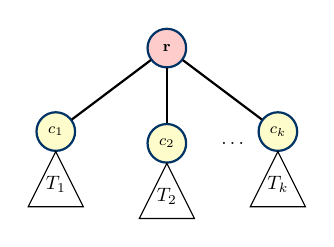
\begin{tikzpicture}[scale=0.7, transform shape]
					\node[treenode, fill=red!20] (r) {r};
					\node[treenode, fill=yellow!20] (c1) [below left=of r, xshift=-0.5cm] {$c_1$};
					\node[treenode, fill=yellow!20] (c2) [below=of r] {$c_2$};
					\node (dots) [right=of c2, xshift=-0.5cm] {$\dots$};
					\node[treenode, fill=yellow!20] (ck) [below right=of r, xshift=0.5cm] {$c_k$};
					
					\draw[thick] (r) -- (c1);
					\draw[thick] (r) -- (c2);
					\draw[thick] (r) -- (ck);
					
					\draw (c1.south) -- ++(-0.5,-1) -- ++(1,0) -- cycle;
					\node at ($(c1.south)+(0,-0.6)$) {$T_1$};
					
					\draw (c2.south) -- ++(-0.5,-1) -- ++(1,0) -- cycle;
					\node at ($(c2.south)+(0,-0.6)$) {$T_2$};
					
					\draw (ck.south) -- ++(-0.5,-1) -- ++(1,0) -- cycle;
					\node at ($(ck.south)+(0,-0.6)$) {$T_k$};
				\end{tikzpicture}
			\end{column}
		\end{columns}
	\end{frame}

    \begin{frame}[t]{1. ĐỊNH NGHĨA VÀ CÁC KHÁI NIỆM CHUNG}
    \vspace{0.1cm}
    \begin{itemize}
        \item \textbf{1.1. Định nghĩa cây}
        \item Ví dụ cây thực tế trong các ứng dụng
    \end{itemize}

    \vspace{0.05cm}
    \centering
    % Ép nhỏ xuống còn 65% chiều rộng trang
    \resizebox{0.65\textwidth}{!}{%
    \begin{tikzpicture}[
        grow=left,
        % --- SIẾT CHẶT KHOẢNG CÁCH HƠN NỮA ---
        level 1/.style={sibling distance=1.2cm, level distance=2.2cm},
        level 2/.style={sibling distance=0.6cm, level distance=2.2cm},
        level 3/.style={sibling distance=0.35cm, level distance=1.5cm},
        edge from parent/.style={draw, HUSTBlue, thick},
        % --- NÚT VÀ CHỮ ---
        dot/.style={circle, draw, thick, inner sep=0pt, minimum size=3.5pt},
        dot_blue/.style={dot, fill=HUSTBlue, draw=HUSTBlue},
        dot_red/.style={dot, fill=red, draw=red},
        winner/.style={circle, draw=black, fill=red, text=yellow, font=\bfseries\tiny, inner sep=0.5pt, minimum size=0.8cm},
        txt/.style={font=\bfseries\tiny, inner sep=1pt},
        txt_blue/.style={txt, text=HUSTBlue},
        txt_red/.style={txt, text=red}
    ]

        % --- CẤU TRÚC CÂY ---
        \node[winner] {Italia}
            child { node[dot_red, label={[txt_red, yshift=-0.5mm]below:Italia}] {}
                child { node[dot_red, label={[txt_red]left:Aghentina}] {} }
                child { node[dot_blue, label={[txt_blue]left:Italia}] {} }
            }
            child { node[dot_blue, label={[txt_blue, yshift=0.5mm]above:Đức}] {}
                child { node[dot_red, label={[txt_red]left:Ucraina}] {} }
                child { node[dot_blue, label={[txt_blue]left:Đức}] {} }
            }
            child { node[dot_blue, label={[txt_blue, yshift=0.5mm]above:Pháp}] {}
                child { node[dot_red, label={[txt_red]left:Anh}] {} }
                child { node[dot_blue, label={[txt_blue]left:Brazin}] {} }
            }
            child { node[dot_blue, label={[txt_blue, yshift=0.5mm]above:Pháp}] {}
                child { node[dot_red, label={[txt_red]left:Tây ban nha}] {} }
                child { node[dot_blue, label={[txt_blue]left:Pháp}] {} }
            };

    \end{tikzpicture}
    }

    \vspace{0.1cm}
    \centering
    \textit{\scriptsize\color{HUSTBlue}
        Diễn tả lịch thi đấu của các giải thể thao theo thể thức đấu loại trực tiếp (World Cup)
    }
\end{frame}

\begin{frame}[t]{1. ĐỊNH NGHĨA VÀ CÁC KHÁI NIỆM CHUNG}
    \vspace{0.1cm}
    \begin{itemize}
        \item \textbf{1.1. Định nghĩa cây}
        \item Ví dụ cây thực tế trong các ứng dụng
    \end{itemize}

    \vspace{0.1cm}
    \centering
    % Resize để cây tự động vừa với slide (chiếm 85% chiều rộng)
    \resizebox{0.85\textwidth}{!}{%
    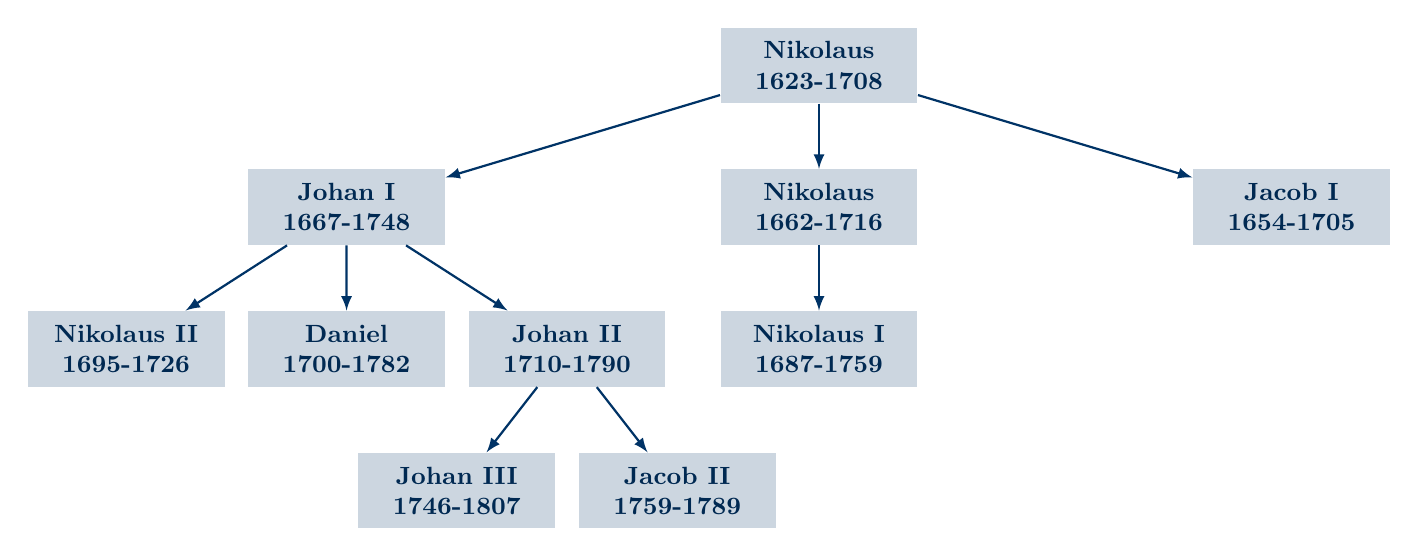
\begin{tikzpicture}[
        % --- CẤU HÌNH KHOẢNG CÁCH ---
        level distance=1.8cm, % Khoảng cách dọc giữa các đời
        % Khoảng cách ngang:
        level 1/.style={sibling distance=6.0cm}, % Đời F1 cần rộng để chứa con cháu
        level 2/.style={sibling distance=2.8cm}, % Đời F2
        level 3/.style={sibling distance=2.8cm}, % Đời F3
        % --- STYLE MŨI TÊN ---
        edge from parent/.style={draw, -latex, thick, HUSTBlue}, % Mũi tên hướng xuống
        % --- STYLE HỘP CHỨA TÊN ---
        person/.style={
            rectangle,
            draw=none,
            fill=HUSTBlue!20, % Màu nền xanh nhạt
            text=HUSTBlue!80!black, % Chữ màu xanh đậm
            align=center,
            font=\bfseries\small,
            inner sep=5pt,
            minimum width=2.5cm
        }
    ]

        % --- GỐC: Nikolaus ---
        \node[person] {Nikolaus\\1623-1708}
            % --- NHÁNH 1: Johan I (Nhánh con đông nhất) ---
            child { node[person] {Johan I\\1667-1748}
                child { node[person] {Nikolaus II\\1695-1726} }
                child { node[person] {Daniel\\1700-1782} }
                child { node[person] {Johan II\\1710-1790}
                    % Cháu của Johan I
                    child { node[person] {Johan III\\1746-1807} }
                    child { node[person] {Jacob II\\1759-1789} }
                }
            }
            % --- NHÁNH 2: Nikolaus ---
            child { node[person] {Nikolaus\\1662-1716}
                child { node[person] {Nikolaus I\\1687-1759} }
            }
            % --- NHÁNH 3: Jacob I ---
            child { node[person] {Jacob I\\1654-1705} };

    \end{tikzpicture}
    }

    \vspace{0.3cm}
    \centering
    \textit{\small\color{HUSTBlue}
        Cây gia phả của các nhà toán học dòng họ Bernoulli
    }
\end{frame}

\begin{frame}[t]{1. ĐỊNH NGHĨA VÀ CÁC KHÁI NIỆM CHUNG}
    \vspace{0.1cm}
    \begin{itemize}
        \item \textbf{1.1. Định nghĩa cây}
        \item Ví dụ cây thực tế trong các ứng dụng
    \end{itemize}

    \vspace{0.3cm}
    \centering
    % Resizebox để đảm bảo sơ đồ rộng vừa khít slide (95% chiều ngang)
    \resizebox{0.95\textwidth}{!}{%
    \begin{tikzpicture}[
        % --- CẤU HÌNH KHOẢNG CÁCH ---
        level distance=1.8cm, % Khoảng cách dọc giữa các cấp
        level 1/.style={sibling distance=3.2cm}, % Khoảng cách giữa các Phòng ban
        level 2/.style={sibling distance=1.4cm}, % Khoảng cách giữa nhân viên/ô trống
        edge from parent/.style={draw, thin}, % Đường nối mảnh, không mũi tên
        % --- STYLE CÁC HỘP ---
        % Style cho Ban giám đốc
        director/.style={
            rectangle, draw, thick,
            minimum width=4cm, minimum height=0.8cm,
            align=center, font=\bfseries\large
        },
        % Style cho các Phòng ban
        dept/.style={
            rectangle, draw, thin,
            minimum width=2.5cm, minimum height=1.2cm,
            align=center, font=\bfseries\small
        },
        % Style cho ô nhân viên (nhỏ hơn)
        staff/.style={
            rectangle, draw, thin,
            minimum width=1.2cm, minimum height=0.6cm,
            align=center, font=\footnotesize
        }
    ]

        % --- GỐC: Ban giám đốc ---
        \node[director] {Ban giám đốc}
            % --- NHÁNH 1: Phòng Hành chính ---
            child { node[dept] {Phòng\\Hành chính}
                child { node[staff] {TP} }
                child { node[staff] {Văn thư} }
            }
            % --- NHÁNH 2: Phòng Tổ chức ---
            child { node[dept] {Phòng\\Tổ chức}
                child { node[staff] {} } % Ô trống
                child { node[staff] {} } % Ô trống
            }
            % --- NHÁNH 3: Phòng Tài vụ ---
            child { node[dept] {Phòng\\Tài vụ}
                child { node[staff] {} }
                child { node[staff] {} }
            }
            % --- NHÁNH 4: Phòng Kinh doanh ---
            child { node[dept] {Phòng Kinh\\doanh}
                child { node[staff] {} }
                child { node[staff] {} }
            }
            % --- NHÁNH 5: Phòng Kế hoạch ---
            child { node[dept] {Phòng\\Kế hoạch}
                child { node[staff] {} }
                child { node[staff] {} }
            };

    \end{tikzpicture}
    }

    \vspace{0.5cm}
    \centering
    \textit{\small\color{HUSTBlue}
        Cây phân cấp quản lý hành chính
    }
\end{frame}

\begin{frame}[t]{1. ĐỊNH NGHĨA VÀ CÁC KHÁI NIỆM CHUNG}
    \textbf{1.1. Định nghĩa cây}
    
    \begin{columns}
        \begin{column}{0.5\textwidth}
            \vspace{-8em}
            \begin{itemize}
            \item Ví dụ thực tế trong các ứng dụng
            \end{itemize}
        \end{column}
        \begin{column}{0.5\textwidth}
            \vspace{-8em}
            \centering
            \includegraphics[width=0.85\textwidth]{tree.png}
        \end{column}
    \end{columns}
\end{frame}
\begin{frame}[t]{1. ĐỊNH NGHĨA VÀ CÁC KHÁI NIỆM CHUNG}
    \vspace{0.2cm}
    \begin{itemize}
        \item 1.2. Các thuật ngữ
    \end{itemize}

    \centering
    \vspace{0.2cm}
    
    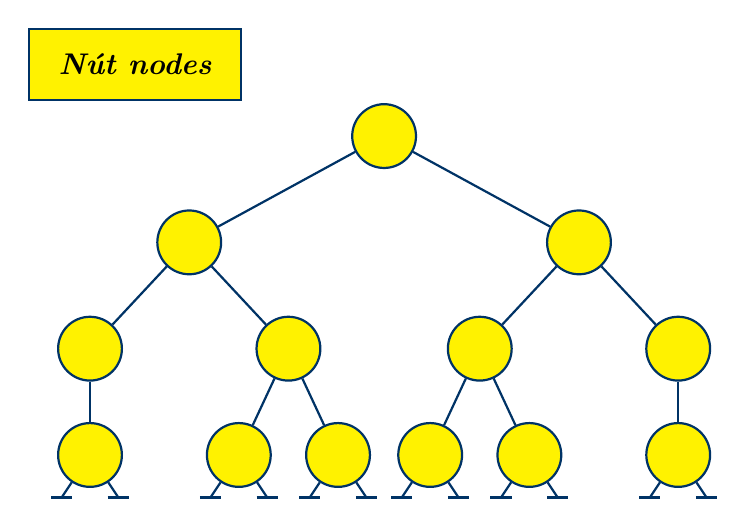
\begin{tikzpicture}[
        scale=0.9, transform shape,
        % Style cho các nút
        treenode/.style={
            circle, 
            draw=HUSTBlue, 
            fill=yellow, 
            thick, 
            minimum size=0.9cm, 
            inner sep=0pt
        },
        % Style cho đường nối
        edge from parent/.style={
            draw=HUSTBlue, 
            thick
        },
        % Khoảng cách cây
        level 1/.style={sibling distance=5.5cm, level distance=1.5cm},
        level 2/.style={sibling distance=2.8cm, level distance=1.5cm},
        level 3/.style={sibling distance=1.4cm, level distance=1.5cm},
        % Style cho chân NULL (hình chữ T)
        nullptr/.style={
            draw=HUSTBlue, thick,
            Path/.style={
                to path={
                    (\tikztostart) -- ++(-0.3,-0.6) coordinate (A) 
                    (\tikztostart) -- ++(0.3,-0.6) coordinate (B)
                    (A) +(-0.15,0) -- +(0.15,0)
                    (B) +(-0.15,0) -- +(0.15,0)
                }
            }
        }
    ]

        % --- HỘP TEXT "Nút nodes" ---
        \node[
            rectangle, 
            draw=HUSTBlue, 
            fill=yellow, 
            thick, 
            minimum width=3cm, 
            minimum height=1cm, 
            anchor=south east,
            font=\bfseries\large\itshape
        ] at (-2, 0.5) {Nút nodes};

        % --- CẤU TRÚC CÂY ---
        \node[treenode] (root) {}
            % Nhánh Trái
            child { node[treenode] {} 
                child { node[treenode] {} 
                    child { node[treenode] (L1) {} } % Lá
                }
                child { node[treenode] {} 
                    child { node[treenode] (L2) {} } % Lá
                    child { node[treenode] (L3) {} } % Lá
                }
            }
            % Nhánh Phải
            child { node[treenode] {}
                child { node[treenode] {}
                    child { node[treenode] (L4) {} } % Lá
                    child { node[treenode] (L5) {} } % Lá
                }
                child { node[treenode] {}
                    child { node[treenode] (L6) {} } % Lá
                }
            };

        % --- VẼ CÁC CHÂN NULL (T-SHAPE) CHO CÁC LÁ ---
        \foreach \leaf in {L1, L2, L3, L4, L5, L6} {
            \draw[HUSTBlue, thick] (\leaf) -- ++(-0.4,-0.6) coordinate (A);
            \draw[HUSTBlue, thick] (A) +(-0.15,0) -- +(0.15,0); % Gạch ngang trái
            
            \draw[HUSTBlue, thick] (\leaf) -- ++(0.4,-0.6) coordinate (B);
            \draw[HUSTBlue, thick] (B) +(-0.15,0) -- +(0.15,0); % Gạch ngang phải
        }

    \end{tikzpicture}
\end{frame}

\begin{frame}[t]{1. ĐỊNH NGHĨA VÀ CÁC KHÁI NIỆM CHUNG}
    \vspace{0.2cm}
    \begin{itemize}
        \item 1.2. Các thuật ngữ
    \end{itemize}

    \centering
    \vspace{0.2cm}
    
    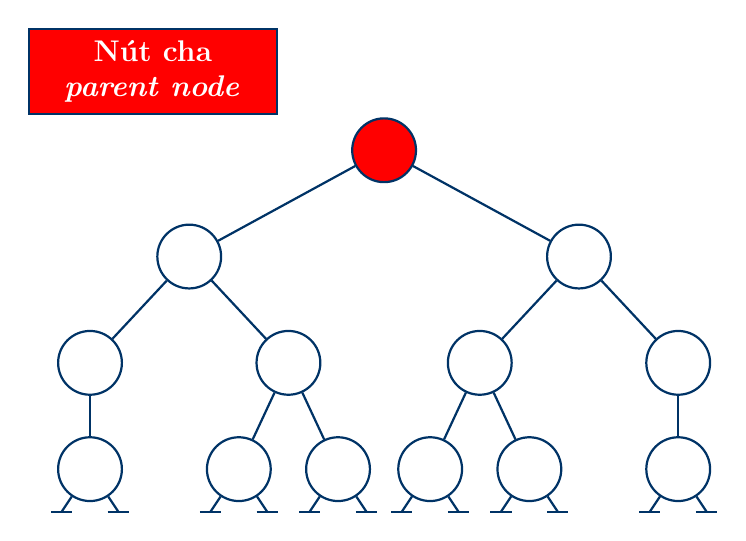
\begin{tikzpicture}[
        scale=0.9, transform shape,
        % Style chung cho nút
        common/.style={
            circle, 
            draw=HUSTBlue, 
            thick, 
            minimum size=0.9cm, 
            inner sep=0pt
        },
        % Style cho Nút Cha (Gốc) - Màu đỏ
        parent_node/.style={
            common,
            fill=red
        },
        % Style cho Nút Con/Cháu - Màu trắng
        child_node/.style={
            common,
            fill=white
        },
        % Style cho đường nối
        edge from parent/.style={
            draw=HUSTBlue, 
            thick
        },
        % Khoảng cách cây
        level 1/.style={sibling distance=5.5cm, level distance=1.5cm},
        level 2/.style={sibling distance=2.8cm, level distance=1.5cm},
        level 3/.style={sibling distance=1.4cm, level distance=1.5cm}
    ]

        % --- HỘP TEXT "Nút cha / parent node" ---
        \node[
            rectangle, 
            draw=HUSTBlue,      % Viền xanh mảnh
            fill=red,           % Nền đỏ
            text=white,         % Chữ trắng
            thick, 
            align=center,       % Căn giữa để xuống dòng
            minimum width=3.5cm, 
            minimum height=1.2cm, 
            anchor=south east,
            font=\bfseries\large
        ] at (-1.5, 0.5) {Nút cha \\ \textit{parent node}};

        % --- CẤU TRÚC CÂY ---
        % Nút gốc dùng style 'parent_node' (Đỏ)
        \node[parent_node] (root) {}
            % Các nút con dùng style 'child_node' (Trắng)
            child { node[child_node] {} 
                child { node[child_node] {} 
                    child { node[child_node] (L1) {} } 
                }
                child { node[child_node] {} 
                    child { node[child_node] (L2) {} } 
                    child { node[child_node] (L3) {} } 
                }
            }
            child { node[child_node] {}
                child { node[child_node] {}
                    child { node[child_node] (L4) {} } 
                    child { node[child_node] (L5) {} } 
                }
                child { node[child_node] {}
                    child { node[child_node] (L6) {} } 
                }
            };

        % --- VẼ CHÂN NULL CHO CÁC LÁ ---
        \foreach \leaf in {L1, L2, L3, L4, L5, L6} {
            \draw[HUSTBlue, thick] (\leaf) -- ++(-0.4,-0.6) coordinate (A);
            \draw[HUSTBlue, thick] (A) +(-0.15,0) -- +(0.15,0);
            
            \draw[HUSTBlue, thick] (\leaf) -- ++(0.4,-0.6) coordinate (B);
            \draw[HUSTBlue, thick] (B) +(-0.15,0) -- +(0.15,0);
        }

    \end{tikzpicture}
\end{frame}
\begin{frame}[t]{1. ĐỊNH NGHĨA VÀ CÁC KHÁI NIỆM CHUNG}
    \vspace{0.2cm}
    \begin{itemize}
        \item 1.2. Các thuật ngữ
    \end{itemize}

    \centering
    \vspace{0.2cm}
    
    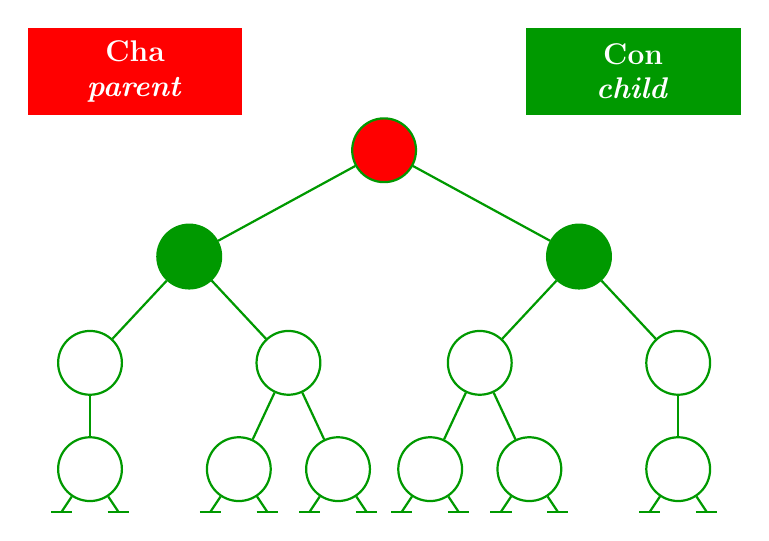
\begin{tikzpicture}[
        scale=0.9, transform shape,
        % --- STYLE CHUNG ---
        common/.style={
            circle, 
            draw=green!60!black, % Viền xanh lá đậm
            thick, 
            minimum size=0.9cm, 
            inner sep=0pt
        },
        % Style Cha (Đỏ)
        parent_node/.style={
            common,
            fill=red
        },
        % Style Con (Xanh lá đậm)
        child_node_active/.style={
            common,
            fill=green!60!black
        },
        % Style Cháu (Trắng)
        other_node/.style={
            common,
            fill=white
        },
        % Style đường nối
        edge from parent/.style={
            draw=green!60!black, 
            thick
        },
        % Khoảng cách cây
        level 1/.style={sibling distance=5.5cm, level distance=1.5cm},
        level 2/.style={sibling distance=2.8cm, level distance=1.5cm},
        level 3/.style={sibling distance=1.4cm, level distance=1.5cm}
    ]

        % --- HỘP TEXT "Cha / parent" ---
        \node[
            rectangle, 
            draw=red, 
            fill=red, 
            text=white, 
            thick, 
            align=center, 
            minimum width=3cm, 
            minimum height=1.2cm, 
            anchor=south east,
            font=\bfseries\large
        ] at (-2, 0.5) {Cha \\ \textit{parent}};

        % --- HỘP TEXT "Con / child" ---
        \node[
            rectangle, 
            draw=green!60!black, 
            fill=green!60!black, 
            text=white, 
            thick, 
            align=center, 
            minimum width=3cm, 
            minimum height=1.2cm, 
            anchor=south west,
            font=\bfseries\large
        ] at (2, 0.5) {Con \\ \textit{child}};

        % --- CẤU TRÚC CÂY ---
        % Gốc là Cha -> Màu đỏ
        \node[parent_node] (root) {}
            % Các con trực tiếp -> Màu xanh lá đậm
            child { node[child_node_active] {} 
                child { node[other_node] {} 
                    child { node[other_node] (L1) {} } 
                }
                child { node[other_node] {} 
                    child { node[other_node] (L2) {} } 
                    child { node[other_node] (L3) {} } 
                }
            }
            child { node[child_node_active] {}
                child { node[other_node] {}
                    child { node[other_node] (L4) {} } 
                    child { node[other_node] (L5) {} } 
                }
                child { node[other_node] {}
                    child { node[other_node] (L6) {} } 
                }
            };

        % --- VẼ CHÂN NULL (Màu xanh lá) ---
        \foreach \leaf in {L1, L2, L3, L4, L5, L6} {
            \draw[green!60!black, thick] (\leaf) -- ++(-0.4,-0.6) coordinate (A);
            \draw[green!60!black, thick] (A) +(-0.15,0) -- +(0.15,0);
            
            \draw[green!60!black, thick] (\leaf) -- ++(0.4,-0.6) coordinate (B);
            \draw[green!60!black, thick] (B) +(-0.15,0) -- +(0.15,0);
        }

    \end{tikzpicture}
\end{frame}
\begin{frame}[t]{1. ĐỊNH NGHĨA VÀ CÁC KHÁI NIỆM CHUNG}
    \vspace{0.2cm}
    \begin{itemize}
        \item 1.2. Các thuật ngữ
    \end{itemize}

    \centering
    \vspace{0.2cm}
    
    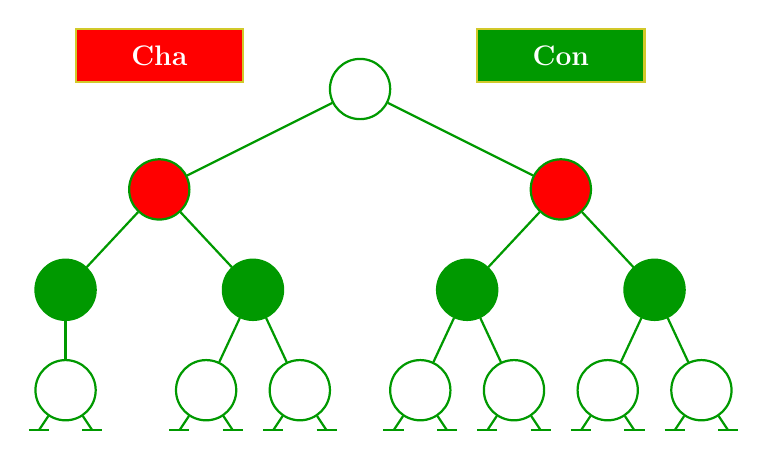
\begin{tikzpicture}[
        scale=0.85, transform shape,
        % --- MÀU SẮC ---
        mygreen/.style={color=green!60!black},
        % --- STYLE CHUNG ---
        common/.style={
            circle, 
            draw=green!60!black,
            thick, 
            minimum size=0.9cm, 
            inner sep=0pt
        },
        % Style Nút Gốc & Lá (Trắng)
        white_node/.style={
            common,
            fill=white
        },
        % Style Nút Cha (Đỏ)
        parent_node/.style={
            common,
            fill=red
        },
        % Style Nút Con (Xanh lá)
        child_node/.style={
            common,
            fill=green!60!black
        },
        % Style đường nối (Xanh lá)
        edge from parent/.style={
            draw=green!60!black, 
            thick
        },
        % Khoảng cách cây
        level 1/.style={sibling distance=6.0cm, level distance=1.5cm},
        level 2/.style={sibling distance=2.8cm, level distance=1.5cm},
        level 3/.style={sibling distance=1.4cm, level distance=1.5cm}
    ]

        % --- HỘP TEXT "Cha" ---
        \node[
            rectangle, 
            draw=yellow!80!black,
            fill=red, 
            text=white, 
            thick, 
            align=center, 
            minimum width=2.5cm, 
            minimum height=0.8cm, 
            font=\bfseries\large
        ] at (-3, 0.5) {Cha};

        % --- HỘP TEXT "Con" ---
        \node[
            rectangle, 
            draw=yellow!80!black,
            fill=green!60!black, 
            text=white, 
            thick, 
            align=center, 
            minimum width=2.5cm, 
            minimum height=0.8cm, 
            font=\bfseries\large
        ] at (3, 0.5) {Con};

        % --- CẤU TRÚC CÂY ---
        \node[white_node] (root) {}
            % CẤP 1: CHA (MÀU ĐỎ)
            child { node[parent_node] {} 
                % CẤP 2: CON (MÀU XANH)
                child { node[child_node] {} 
                    % CẤP 3: LÁ (TRẮNG)
                    child { node[white_node] (L1) {} } 
                }
                child { node[child_node] {} 
                    child { node[white_node] (L2) {} } 
                    child { node[white_node] (L3) {} } 
                }
            }
            % CẤP 1: CHA (MÀU ĐỎ)
            child { node[parent_node] {}
                % CẤP 2: CON (MÀU XANH)
                child { node[child_node] {}
                    child { node[white_node] (L4) {} } 
                    child { node[white_node] (L5) {} } 
                }
                child { node[child_node] {}
                    child { node[white_node] (L6) {} } 
                    child { node[white_node] (L7) {} }
                }
            };

        % --- VẼ CHÂN NULL (Màu xanh lá) ---
        \foreach \leaf in {L1, L2, L3, L4, L5, L6, L7} {
            \draw[green!60!black, thick] (\leaf) -- ++(-0.4,-0.6) coordinate (A);
            \draw[green!60!black, thick] (A) +(-0.15,0) -- +(0.15,0);
            \draw[green!60!black, thick] (\leaf) -- ++(0.4,-0.6) coordinate (B);
            \draw[green!60!black, thick] (B) +(-0.15,0) -- +(0.15,0);
        }

    \end{tikzpicture}
\end{frame}

\begin{frame}[t]{1. ĐỊNH NGHĨA VÀ CÁC KHÁI NIỆM CHUNG}
    \vspace{0.2cm}
    \begin{itemize}
        \item 1.2. Các thuật ngữ
    \end{itemize}

    \centering
    \vspace{0.2cm}
    
    \begin{tikzpicture}[
        scale=0.85, transform shape,
        % --- STYLE CHUNG ---
        common/.style={
            circle, 
            draw=green!60!black, % Viền xanh lá đậm
            thick, 
            minimum size=0.9cm, 
            inner sep=0pt
        },
        % Style Nút Gốc (Hồng)
        root_node/.style={
            common,
            fill=magenta!50
        },
        % Style Nút Lá (Tím)
        leaf_node/.style={
            common,
            fill=violet
        },
        % Style Nút Trong (Trắng)
        internal_node/.style={
            common,
            fill=white
        },
        % Style đường nối (Xanh lá)
        edge from parent/.style={
            draw=green!60!black, 
            thick
        },
        % Khoảng cách cây
        level 1/.style={sibling distance=6.0cm, level distance=1.5cm},
        level 2/.style={sibling distance=2.8cm, level distance=1.5cm},
        level 3/.style={sibling distance=1.4cm, level distance=1.5cm}
    ]

        % --- HỘP TEXT "Gốc - root" ---
        \node[
            rectangle, 
            draw=green!60!black, % Viền xanh
            fill=magenta!50,     % Nền hồng
            text=black,          % Chữ đen
            thick, 
            align=center, 
            minimum width=3cm, 
            minimum height=0.8cm, 
            font=\bfseries\large
        ] at (-3, 0.5) {Gốc - \textit{root}};

        % --- HỘP TEXT "Lá - leaf" ---
        \node[
            rectangle, 
            draw=green!60!black, % Viền xanh
            fill=violet,         % Nền tím
            text=white,          % Chữ trắng
            thick, 
            align=center, 
            minimum width=3cm, 
            minimum height=0.8cm, 
            font=\bfseries\large
        ] at (3, 0.5) {Lá - \textit{leaf}};

        % --- CẤU TRÚC CÂY ---
        % Gốc màu hồng
        \node[root_node] (root) {}
            % Nhánh Trái
            child { node[internal_node] {} 
                child { node[internal_node] {} 
                    child { node[leaf_node] (L1) {} } % Lá
                }
                child { node[internal_node] {} 
                    child { node[leaf_node] (L2) {} } % Lá
                    child { node[leaf_node] (L3) {} } % Lá
                }
            }
            % Nhánh Phải
            child { node[internal_node] {}
                child { node[internal_node] {}
                    child { node[leaf_node] (L4) {} } % Lá
                    child { node[leaf_node] (L5) {} } % Lá
                }
                child { node[internal_node] {}
                    child { node[leaf_node] (L6) {} } % Lá
                    child { node[leaf_node] (L7) {} } % Lá
                }
            };

        % --- VẼ CHÂN NULL (Màu xanh lá) ---
        \foreach \leaf in {L1, L2, L3, L4, L5, L6, L7} {
            \draw[green!60!black, thick] (\leaf) -- ++(-0.4,-0.6) coordinate (A);
            \draw[green!60!black, thick] (A) +(-0.15,0) -- +(0.15,0);
            \draw[green!60!black, thick] (\leaf) -- ++(0.4,-0.6) coordinate (B);
            \draw[green!60!black, thick] (B) +(-0.15,0) -- +(0.15,0);
        }

    \end{tikzpicture}
\end{frame}
\begin{frame}[t]{1. ĐỊNH NGHĨA VÀ CÁC KHÁI NIỆM CHUNG}
    \vspace{0.2cm}
    \begin{itemize}
        \item 1.2. Các thuật ngữ
    \end{itemize}

    \centering
    \vspace{0.5cm} % Tăng khoảng cách một chút để hộp text không đè lên tiêu đề
    
    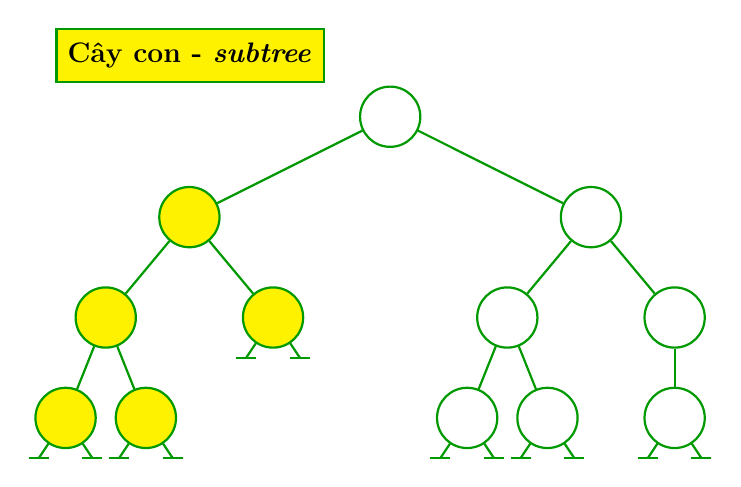
\begin{tikzpicture}[
        scale=0.85, transform shape,
        % --- STYLE CHUNG ---
        common/.style={
            circle, 
            draw=green!60!black, % Viền xanh lá đậm
            thick, 
            minimum size=0.9cm, 
            inner sep=0pt
        },
        % Style Nút Nổi bật (Vàng - Cây con)
        highlight_node/.style={
            common,
            fill=yellow
        },
        % Style Nút Thường (Trắng)
        normal_node/.style={
            common,
            fill=white
        },
        % Style đường nối (Xanh lá)
        edge from parent/.style={
            draw=green!60!black, 
            thick
        },
        % Khoảng cách cây
        level 1/.style={sibling distance=6.0cm, level distance=1.5cm},
        level 2/.style={sibling distance=2.5cm, level distance=1.5cm},
        level 3/.style={sibling distance=1.2cm, level distance=1.5cm}
    ]

        % --- HỘP TEXT "Cây con - subtree" ---
        \node[
            rectangle, 
            draw=green!60!black, % Viền xanh
            fill=yellow,         % Nền vàng
            text=black,          % Chữ đen
            thick, 
            align=center, 
            minimum width=4cm, 
            minimum height=0.8cm, 
            font=\bfseries\large,
            anchor=south west
        ] at (-5, 0.5) {Cây con - \textit{subtree}};

        % --- CẤU TRÚC CÂY ---
        % Gốc (Trắng)
        \node[normal_node] (root) {}
            % --- NHÁNH TRÁI (CÂY CON - MÀU VÀNG) ---
            child { node[highlight_node] {} 
                % Con trái của cây con (Vàng) -> Có 2 lá
                child { node[highlight_node] {} 
                    child { node[highlight_node] (L1) {} } 
                    child { node[highlight_node] (L2) {} } 
                }
                % Con phải của cây con (Vàng) -> Là lá
                child { node[highlight_node] (L3) {} } 
            }
            % --- NHÁNH PHẢI (TRẮNG) ---
            child { node[normal_node] {}
                % Con trái (Trắng) -> Có 2 lá
                child { node[normal_node] {}
                    child { node[normal_node] (L4) {} } 
                    child { node[normal_node] (L5) {} } 
                }
                % Con phải (Trắng) -> Có 1 lá
                child { node[normal_node] {}
                    child { node[normal_node] (L6) {} } 
                }
            };

        % --- VẼ CHÂN NULL (Màu xanh lá) ---
        % Lặp qua danh sách các nút lá để vẽ chân T
        \foreach \leaf in {L1, L2, L3, L4, L5, L6} {
            \draw[green!60!black, thick] (\leaf) -- ++(-0.4,-0.6) coordinate (A);
            \draw[green!60!black, thick] (A) +(-0.15,0) -- +(0.15,0);
            
            \draw[green!60!black, thick] (\leaf) -- ++(0.4,-0.6) coordinate (B);
            \draw[green!60!black, thick] (B) +(-0.15,0) -- +(0.15,0);
        }

    \end{tikzpicture}
\end{frame}

\begin{frame}[t]{1. ĐỊNH NGHĨA VÀ CÁC KHÁI NIỆM CHUNG}
    \vspace{0.2cm}
    \begin{itemize}
        \item 1.2. Các thuật ngữ
    \end{itemize}

    \centering
    \vspace{0.5cm}
    
    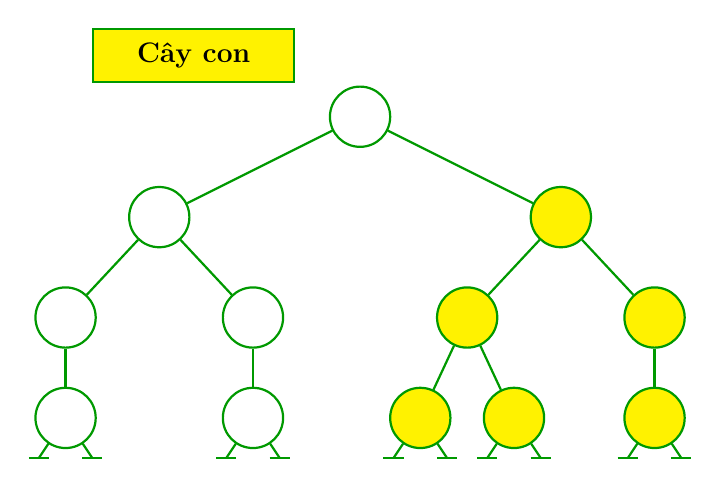
\begin{tikzpicture}[
        scale=0.85, transform shape,
        % --- STYLE CHUNG ---
        common/.style={
            circle, 
            draw=green!60!black, % Viền xanh lá đậm
            thick, 
            minimum size=0.9cm, 
            inner sep=0pt
        },
        % Style Nút Nổi bật (Vàng)
        highlight_node/.style={
            common,
            fill=yellow
        },
        % Style Nút Thường (Trắng)
        normal_node/.style={
            common,
            fill=white
        },
        % Style đường nối (Xanh lá)
        edge from parent/.style={
            draw=green!60!black, 
            thick
        },
        % Khoảng cách cây
        level 1/.style={sibling distance=6.0cm, level distance=1.5cm},
        level 2/.style={sibling distance=2.8cm, level distance=1.5cm},
        level 3/.style={sibling distance=1.4cm, level distance=1.5cm}
    ]

        % --- HỘP TEXT "Cây con" ---
        \node[
            rectangle, 
            draw=green!60!black, 
            fill=yellow, 
            text=black, 
            thick, 
            align=center, 
            minimum width=3cm, 
            minimum height=0.8cm, 
            font=\bfseries\large,
            anchor=south west
        ] at (-4, 0.5) {Cây con};

        % --- CẤU TRÚC CÂY ---
        % Gốc (Trắng)
        \node[normal_node] (root) {}
            % --- NHÁNH TRÁI (TRẮNG) ---
            child { node[normal_node] {} 
                child { node[normal_node] {} 
                    child { node[normal_node] (L1) {} } 
                }
                child { node[normal_node] {} 
                    child { node[normal_node] (L2) {} } 
                }
            }
            % --- NHÁNH PHẢI (CÂY CON - MÀU VÀNG) ---
            child { node[highlight_node] {}
                % Con trái của cây con (Vàng) -> Có 2 lá
                child { node[highlight_node] {}
                    child { node[highlight_node] (L3) {} } 
                    child { node[highlight_node] (L4) {} } 
                }
                % Con phải của cây con (Vàng) -> Có 1 lá
                child { node[highlight_node] {}
                    child { node[highlight_node] (L5) {} } 
                }
            };

        % --- VẼ CHÂN NULL (Màu xanh lá) ---
        \foreach \leaf in {L1, L2, L3, L4, L5} {
            \draw[green!60!black, thick] (\leaf) -- ++(-0.4,-0.6) coordinate (A);
            \draw[green!60!black, thick] (A) +(-0.15,0) -- +(0.15,0);
            
            \draw[green!60!black, thick] (\leaf) -- ++(0.4,-0.6) coordinate (B);
            \draw[green!60!black, thick] (B) +(-0.15,0) -- +(0.15,0);
        }

    \end{tikzpicture}
\end{frame}

\begin{frame}[t]{1. ĐỊNH NGHĨA VÀ CÁC KHÁI NIỆM CHUNG}
    \vspace{0.2cm}
    \begin{itemize}
        \item 1.2. Các thuật ngữ
    \end{itemize}

    \centering
    \vspace{0.5cm}
    
    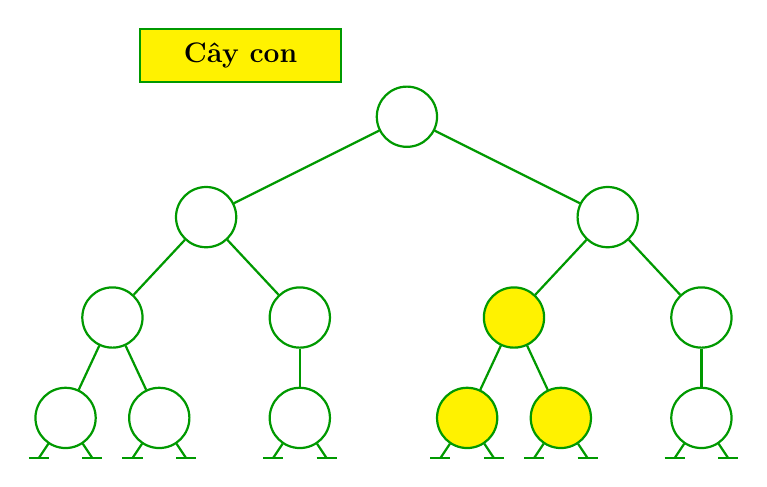
\begin{tikzpicture}[
        scale=0.85, transform shape,
        % --- STYLE CHUNG ---
        common/.style={
            circle, 
            draw=green!60!black, % Viền xanh lá đậm
            thick, 
            minimum size=0.9cm, 
            inner sep=0pt
        },
        % Style Nút Nổi bật (Vàng)
        highlight_node/.style={
            common,
            fill=yellow
        },
        % Style Nút Thường (Trắng)
        normal_node/.style={
            common,
            fill=white
        },
        % Style đường nối (Xanh lá)
        edge from parent/.style={
            draw=green!60!black, 
            thick
        },
        % Khoảng cách cây
        level 1/.style={sibling distance=6.0cm, level distance=1.5cm},
        level 2/.style={sibling distance=2.8cm, level distance=1.5cm},
        level 3/.style={sibling distance=1.4cm, level distance=1.5cm}
    ]

        % --- HỘP TEXT "Cây con" ---
        \node[
            rectangle, 
            draw=green!60!black, 
            fill=yellow, 
            text=black, 
            thick, 
            align=center, 
            minimum width=3cm, 
            minimum height=0.8cm, 
            font=\bfseries\large,
            anchor=south west
        ] at (-4, 0.5) {Cây con};

        % --- CẤU TRÚC CÂY ---
        % Gốc (Trắng)
        \node[normal_node] (root) {}
            % --- NHÁNH TRÁI (TRẮNG) ---
            child { node[normal_node] {} 
                child { node[normal_node] {} 
                    child { node[normal_node] (L1) {} } 
                    child { node[normal_node] (L2) {} } 
                }
                child { node[normal_node] {} 
                    child { node[normal_node] (L3) {} } 
                }
            }
            % --- NHÁNH PHẢI ---
            child { node[normal_node] {} % Nút cha của cây con (Trắng)
                % === CÂY CON ĐƯỢC CHỌN (MÀU VÀNG) ===
                child { node[highlight_node] {} 
                    child { node[highlight_node] (L4) {} } 
                    child { node[highlight_node] (L5) {} } 
                }
                % Con phải còn lại (Trắng)
                child { node[normal_node] {}
                    child { node[normal_node] (L6) {} } 
                }
            };

        % --- VẼ CHÂN NULL (Màu xanh lá) ---
        \foreach \leaf in {L1, L2, L3, L4, L5, L6} {
            \draw[green!60!black, thick] (\leaf) -- ++(-0.4,-0.6) coordinate (A);
            \draw[green!60!black, thick] (A) +(-0.15,0) -- +(0.15,0);
            
            \draw[green!60!black, thick] (\leaf) -- ++(0.4,-0.6) coordinate (B);
            \draw[green!60!black, thick] (B) +(-0.15,0) -- +(0.15,0);
        }

    \end{tikzpicture}
\end{frame}

\begin{frame}[t]{1. ĐỊNH NGHĨA VÀ CÁC KHÁI NIỆM CHUNG}
    \vspace{0.2cm}
    \begin{itemize}
        \item 1.2. Các thuật ngữ
    \end{itemize}

    \centering
    \vspace{0.1cm}
    
    \begin{tikzpicture}[
        scale=0.85, transform shape,
        % --- STYLE ---
        % Style cho nút: Tròn, nền xanh, chữ vàng
        treenode/.style={
            circle, 
            draw=black!50, 
            fill=HUSTBlue!80, 
            text=yellow, 
            font=\bfseries,
            minimum size=0.8cm, 
            inner sep=0pt
        },
        % Style đường nối thường
        normalline/.style={
            draw=black!60, 
            thin
        },
        % Style đường nối nổi bật (Path)
        pathline/.style={
            draw=magenta, 
            line width=2pt
        },
        % Khoảng cách cây
        level 1/.style={sibling distance=4.5cm, level distance=1.5cm},
        level 2/.style={sibling distance=2.2cm, level distance=1.5cm},
        level 3/.style={sibling distance=1.5cm, level distance=1.5cm}
    ]

        % --- VẼ CÂY & ĐẶT TÊN NÚT (a,b,c...) ---
        \node[treenode] (a) {a}
            % Nhánh b
            child { node[treenode] (b) {b}
                child { node[treenode] (e) {e} edge from parent[normalline] }
                child { node[treenode] (f) {f} 
                    child { node[treenode] (j) {j} edge from parent[normalline] } % Tạm vẽ thường, sẽ đè path sau
                    edge from parent[normalline]
                }
                edge from parent[normalline]
            }
            % Nhánh c
            child { node[treenode] (c) {c}
                child { node[treenode] (g) {g} edge from parent[normalline] }
                edge from parent[normalline]
            }
            % Nhánh d
            child { node[treenode] (d) {d}
                child { node[treenode] (h) {h} edge from parent[normalline] }
                child { node[treenode] (i) {i} edge from parent[normalline] }
                edge from parent[normalline]
            };

        % --- VẼ ĐÈ CÁC ĐƯỜNG PATH (MÀU HỒNG) ---
        % Path 1: a -> b -> f -> j
        \draw[pathline] (a) -- (b);
        \draw[pathline] (b) -- (f);
        \draw[pathline] (f) -- (j);
        
        % Path 2: d -> i
        \draw[pathline] (d) -- (i);

        % --- CHÚ THÍCH TRÊN CÂY ---
        % Label Path 1
        \node[text=blue, font=\footnotesize, right=0.1cm] at ($(b)!0.5!(f)$) {Path 1};
        % Label Path 2
        \node[text=blue, font=\footnotesize, right=0.1cm] at ($(d)!0.5!(i)$) {Path 2};

        % --- CÁC HỘP TEXT GIẢI THÍCH ---
        % Text bên trái (Tím)
        \node[text=violet, align=left, font=\bfseries\footnotesize, anchor=south east] 
            at ($(a)+(-2.5,0)$) 
            {Từ cha đến con và đến\\các nút hậu duệ};
            
        % Text bên phải (Cam)
        \node[text=orange, align=left, font=\bfseries\footnotesize, anchor=south west] 
            at ($(a)+(2.5,0)$) 
            {Có duy nhất 1 đường đi từ\\một nút đến một nút là\\hậu duệ của nó};

        % Text liệt kê Path (Xanh dương)
        \node[text=blue, align=left, font=\bfseries\small, anchor=north west] 
            at (2, -4.5) 
            {Path 1: $\{ a, b, f, j \}$\\Path 2: $\{ d, i \}$};

        % Caption
        \node[text=HUSTBlue!70, font=\itshape\large] at (0, -5.5) {Đường đi trên cây};

    \end{tikzpicture}
\end{frame}

\begin{frame}[t]{1. ĐỊNH NGHĨA VÀ CÁC KHÁI NIỆM CHUNG}
    \vspace{0.2cm}
    \begin{itemize}
        \item 1.2. Các thuật ngữ
    \end{itemize}

    \centering
    \vspace{0.1cm}
    
    % Thu nhỏ khung hình xuống 80% chiều rộng văn bản
    \resizebox{0.8\textwidth}{!}{%
    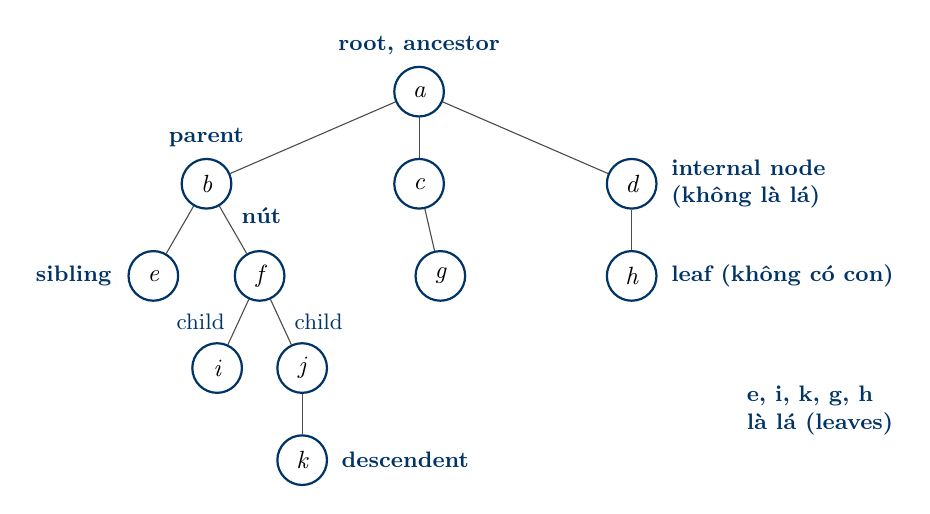
\begin{tikzpicture}[
        scale=0.9, transform shape,
        % --- STYLE ---
        treenode/.style={
            circle, 
            draw=HUSTBlue, 
            thick, 
            minimum size=0.7cm, 
            inner sep=0pt,
            font=\itshape
        },
        edge from parent/.style={
            draw=black!70, 
            thin
        },
        % Style cho text chú thích
        label_text/.style={
            text=HUSTBlue,
            font=\small\bfseries,
            align=left % Bắt buộc có để dùng \\
        },
        % Khoảng cách cây (Đã thu gọn bớt)
        level 1/.style={sibling distance=3.0cm, level distance=1.3cm},
        level 2/.style={sibling distance=1.5cm, level distance=1.3cm},
        level 3/.style={sibling distance=1.2cm, level distance=1.3cm},
        level 4/.style={sibling distance=1.2cm, level distance=1.3cm}
    ]

        % --- VẼ CÂY ---
        \node[treenode] (a) {a}
            % Nhánh b
            child { node[treenode] (b) {b}
                child { node[treenode] (e) {e} }
                child { node[treenode] (f) {f}
                    % Nhánh i
                    child { node[treenode] (i) {i} 
                        edge from parent node[left, xshift=-2pt, font=\small, text=HUSTBlue] {child}
                    }
                    % Nhánh j
                    child { node[treenode] (j) {j}
                        child { node[treenode] (k) {k} }
                        edge from parent node[right, xshift=2pt, font=\small, text=HUSTBlue] {child}
                    }
                }
            }
            % Nhánh c
            child { node[treenode] (c) {c}
                child { node[treenode, xshift=0.3cm] (g) {g} } % Dịch ít hơn
            }
            % Nhánh d
            child { node[treenode] (d) {d}
                child { node[treenode] (h) {h} }
            };

        % --- CÁC CHÚ THÍCH (LABELS) ---
        
        \node[label_text, above=1pt] at (a.north) {root, ancestor};
        \node[label_text, above=1pt] at (b.north) {parent};
        \node[label_text, left=3pt] at (e.west) {sibling};
        
        % Chỉnh lại vị trí label "nút"
        \node[label_text] at ($(b)!0.5!(f) + (0.4, 0.2)$) {nút};
        
        \node[label_text, right=2pt] at (d.east) {internal node\\(không là lá)};
        \node[label_text, right=2pt] at (h.east) {leaf (không có con)};
        \node[label_text, right=2pt] at (k.east) {descendent};
        
        % --- SỬA LỖI BIÊN DỊCH Ở ĐÂY ---
        % Thêm align=left để fix lỗi "Not allowed in LR mode"
        \node[text=HUSTBlue, font=\small\bfseries, anchor=west, align=left] at (4.5, -4.5) 
            {e, i, k, g, h\\là lá (leaves)};

    \end{tikzpicture}
    }
    
    \vspace{0.1cm}
    \textit{\small\color{HUSTBlue} Các thuật ngữ với cây có gốc}
\end{frame}

\begin{frame}[t]{1. ĐỊNH NGHĨA VÀ CÁC KHÁI NIỆM CHUNG}
    \vspace{0.1cm}
    
    \textbf{\large Cây có nhãn (Labeled Tree)}
    
    \begin{columns}[T]
        % --- CỘT TRÁI: LÝ THUYẾT ---
        \begin{column}{0.55\textwidth}
            \small
            \begin{itemize}
                \item Mỗi nút của cây 1 nhãn (label) hoặc 1 giá trị.
                \item Nhãn của nút không phải là tên gọi của nút mà là giá trị được cất giữ trong nó.
                \item Ví dụ: Xét cây có 7 nút $n_1, \dots, n_7$. Gán nhãn cho các nút:
                \begin{itemize}
                    \item Nút $n_1$ có nhãn *;
                    \item Nút $n_2$ có nhãn +;
                    \item Nút $n_3$ có nhãn -;
                    \item Nút $n_4, n_6$ có nhãn a;
                    \item Nút $n_5$ có nhãn b;
                    \item Nút $n_7$ có nhãn c.
                \end{itemize}
            \end{itemize}
        \end{column}
        
        % --- CỘT PHẢI: HÌNH VẼ ---
        \begin{column}{0.45\textwidth}
            \centering
            \resizebox{0.95\textwidth}{!}{%
            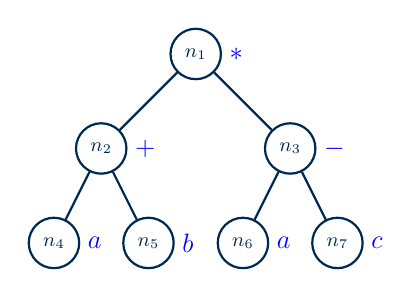
\begin{tikzpicture}[
                scale=0.8, transform shape,
                % Style cho nút (Hình tròn, viền xanh đậm, chữ xanh)
                treenode/.style={
                    circle, 
                    draw=HUSTBlue!80!black, 
                    thick, 
                    text=HUSTBlue!80!black,
                    font=\bfseries\small,
                    minimum size=0.8cm, 
                    inner sep=0pt
                },
                % Style cho nhãn (Label) nằm cạnh nút (Màu xanh nghiêng)
                mylabel/.style={
                    text=blue, 
                    font=\bfseries\large\itshape
                },
                edge from parent/.style={
                    draw=HUSTBlue!80!black, 
                    thick
                },
                level 1/.style={sibling distance=3cm, level distance=1.5cm},
                level 2/.style={sibling distance=1.5cm, level distance=1.5cm}
            ]

                % --- VẼ CÂY ---
                % Gốc n1 (nhãn *)
                \node[treenode, label={[mylabel]0:$*$}] (n1) {$n_1$}
                    % Con trái n2 (nhãn +)
                    child { node[treenode, label={[mylabel]0:$+$}] (n2) {$n_2$}
                        % Con của n2
                        child { node[treenode, label={[mylabel]0:$a$}] (n4) {$n_4$} }
                        child { node[treenode, label={[mylabel]0:$b$}] (n5) {$n_5$} }
                    }
                    % Con phải n3 (nhãn -)
                    child { node[treenode, label={[mylabel]0:$-$}] (n3) {$n_3$}
                        % Con của n3
                        child { node[treenode, label={[mylabel]0:$a$}] (n6) {$n_6$} }
                        child { node[treenode, label={[mylabel]0:$c$}] (n7) {$n_7$} }
                    };

            \end{tikzpicture}
            }
            
            \vspace{0.3cm}
            \textit{\small Cây biểu thức $(a+b)*(a-c)$}
        \end{column}
    \end{columns}
\end{frame}
\section{Cây nhị phân}
\begin{frame}[t]{2. CÂY NHỊ PHÂN}
	\vspace{0.2cm}
	\begin{itemize}
		\item \textbf{2.1. Cây nhị phân}
		\item \textbf{Cây nhị phân (Binary Tree):} Cây mà mỗi nút có nhiều nhất là 2 con
	\end{itemize}
	
	\vspace{0.3cm}
	
	\begin{columns}[T]
		% --- CỘT TRÁI: ĐỊNH NGHĨA ---
		\begin{column}{0.42\textwidth}
			\large
			\begin{itemize}
				\item \textit{Con trái} và \textit{con phải}
				\item Mỗi nút hoặc là:
				\vspace{0.2cm}
				\begin{itemize}
					\item \textcolor{violet}{\textbf{Không có con}}
					\vspace{0.1cm}
					\item \textcolor{red}{\textbf{Chỉ có con trái}}
					\vspace{0.1cm}
					\item \textcolor{blue}{\textbf{Chỉ có con phải}}
					\vspace{0.1cm}
					\item \textcolor{red}{\textbf{Con trái}} và \textcolor{blue}{\textbf{con phải}}
				\end{itemize}
			\end{itemize}
		\end{column}
		
		% --- CỘT PHẢI: HÌNH VẼ MINH HỌA ---
		\begin{column}{0.58\textwidth}
			\centering
			\resizebox{0.95\textwidth}{!}{%
				\begin{tikzpicture}[
					level 1/.style={sibling distance=4.5cm, level distance=1.5cm},
					level 2/.style={sibling distance=2.2cm, level distance=1.8cm},
					level 3/.style={sibling distance=1.0cm, level distance=1.2cm},
					% Style chung cho nút
					treenode/.style={
						circle, 
						draw=HUSTBlue, 
						thick, 
						minimum size=0.9cm, 
						inner sep=0pt
					},
					% Style cho lá (nhỏ hơn, màu trắng)
					leafnode/.style={
						treenode,
						minimum size=0.7cm,
						fill=white
					}
				]
					
					% --- VẼ CÂY ---
					% Gốc (Trắng)
					\node[treenode, fill=white] (root) {}
					% Con Trái (Đỏ)
					child { node[treenode, fill=red] (L) {} 
						child { node[treenode, fill=violet!60] (LL) {} % Hồng/Tím nhạt
							child { node[leafnode] {} }
							child { node[leafnode] {} }
						}
						child { node[treenode, fill=green!60!black] (LR) {} % Xanh lá
							child { node[leafnode] {} }
							child { node[leafnode] {} }
						}
					}
					% Con Phải (Xanh dương đậm)
					child { node[treenode, fill=blue!80!black] (R) {}
						child { node[treenode, fill=yellow] (RL) {} % Vàng
							child { node[leafnode] {} }
							child { node[leafnode] {} }
						}
						child { node[treenode, fill=violet] (RR) {} % Tím đậm
							child { node[leafnode] {} }
							child { node[leafnode] {} }
						}
					};
					
					% --- MŨI TÊN CHÚ THÍCH ---
					% Mũi tên đỏ chỉ vào con trái
					\draw[->, red, line width=3pt] ($(L)+(-2.5, 0.8)$) -- (L) 
					node[pos=0.0, left, font=\bfseries\large, text=red] {Con trái};
					
					% Mũi tên xanh chỉ vào con phải
					\draw[->, blue, line width=3pt] ($(R)+(2.5, 0.8)$) -- (R) 
					node[pos=0.0, right, font=\bfseries\large, text=blue] {Con phải};
					
				\end{tikzpicture}
			}
		\end{column}
	\end{columns}
\end{frame}

\begin{frame}[t]{2. CÂY NHỊ PHÂN}
    \vspace{0.2cm}
    \begin{itemize}
        \item \textbf{2.2. Cây nhị phân đầy đủ}
        \item \textbf{Cây nhị phân đầy đủ (Full Binary Trees):} Cây nhị phân thoả mãn
        \begin{itemize}
            \item Mỗi nút lá đều có cùng độ sâu
            \item Các nút trong có đúng 2 con
        \end{itemize}
    \end{itemize}

    \vspace{0.5cm}
    \centering
    % Resize hình vẽ chiếm 50% chiều rộng slide cho cân đối
    \resizebox{0.5\textwidth}{!}{%
    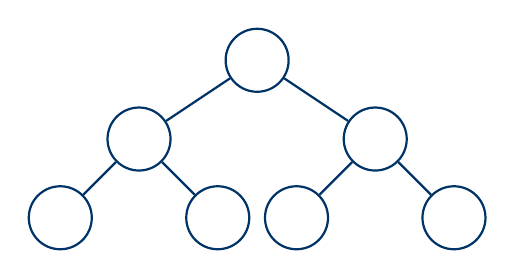
\begin{tikzpicture}[
        % Cấu hình khoảng cách giữa các cấp và các nút anh em
        level 1/.style={sibling distance=3cm, level distance=1cm},
        level 2/.style={sibling distance=2cm, level distance=1cm},
        % Style cho nút: Hình tròn, viền xanh đậm HUST, rỗng
        treenode/.style={
            circle,
            draw=HUSTBlue,
            thick,
            minimum size=0.8cm,
            inner sep=0pt
        },
        % Style đường nối: Xanh đậm, nét dày
        edge from parent/.style={
            draw=HUSTBlue,
            thick
        }
    ]

        % --- VẼ CÂY ---
        % Gốc
        \node[treenode] {}
            % Con trái
            child { node[treenode] {}
                % Các con của con trái (Lá)
                child { node[treenode] {} }
                child { node[treenode] {} }
            }
            % Con phải
            child { node[treenode] {}
                % Các con của con phải (Lá)
                child { node[treenode] {} }
                child { node[treenode] {} }
            };

    \end{tikzpicture}
    }
\end{frame}

\begin{frame}[t]{2. CÂY NHỊ PHÂN}
    \vspace{0.2cm}
    \begin{itemize}
        \item \textbf{2.3. Cây nhị phân hoàn chỉnh}
        \item \textbf{Cây nhị phân hoàn chỉnh (Complete Binary Trees):} Cây nhị phân độ sâu $n$ thoả mãn:
        \begin{itemize}
            \item Là cây nhị phân đầy đủ nếu không tính đến các nút ở độ sâu $n$, và
            \item Tất cả các nút ở độ sâu $n$ là lệch sang trái nhất có thể được.
        \end{itemize}
        \item Cây nhị phân hoàn chỉnh độ sâu $n$ có số lượng nút nằm trong khoảng từ $2^{n-1}$ đến $2^n - 1$
    \end{itemize}

    \vspace{0.2cm}
    \centering
    % Resize hình vẽ vừa vặn
    \resizebox{0.6\textwidth}{!}{%
    \begin{tikzpicture}[
        % Cấu hình khoảng cách cây
        level 1/.style={sibling distance=6.2cm, level distance=1.3cm},
        level 2/.style={sibling distance=3.2cm, level distance=1.2cm},
        level 3/.style={sibling distance=1cm, level distance=0.9cm},
        % Style cho nút: Chấm tròn đen nhỏ
        dot/.style={
            circle,
            fill=black,
            inner sep=0pt,
            minimum size=4pt
        },
        % Style đường nối: Mảnh, màu đen
        edge from parent/.style={
            draw,
            thin
        }
    ]

        % --- VẼ CÂY THEO HÌNH MẪU ---
        % Gốc
        \node[dot] {}
            % --- Nhánh Trái ---
            child { node[dot] {}
                % Con trái: Có 2 lá
                child { node[dot] {}
                    child { node[dot] {}
                    child { node[dot] {} }
                    child { node[dot] {} }
                    }
                    child { node[dot] {}
                    child { node[dot] {} }
                    child { node[dot] {} }
                    }
                }
                % Con phải: Có 1 lá (bên trái)
                child { node[dot] {}
                    child { node[dot] {} 
                    child { node[dot] {} }
                    } 
                    child { node[dot] {} }
                }
            }
            % --- Nhánh Phải (Đối xứng với nhánh trái) ---
            child { node[dot] {}
                % Con trái: Có 2 lá
                child { node[dot] {}
                    child { node[dot] {} }
                    child { node[dot] {} }
                }
                % Con phải: Có 1 lá (bên trái)
                child { node[dot] {}
                    child { node[dot] {} }
                    child { node[dot] {} }
                }
            };

    \end{tikzpicture}
    }
    
    \vspace{0.2cm}
    \textit{\small Cây nhị phân hoàn chỉnh}
\end{frame}

\begin{frame}[t]{2. CÂY NHỊ PHÂN}
    \vspace{0.1cm}
    \begin{itemize}
        \item \textbf{2.4. Cây nhị phân cân đối}
        \item \textbf{Cây nhị phân được gọi là cân đối (balanced)} nếu chiều cao của cây con trái và chiều cao của cây con phải chênh lệch nhau không quá 1 đơn vị
        \item Nhận xét:
        \begin{itemize}
            \item Nếu cây nhị phân là đầy đủ thì nó là hoàn chỉnh
            \item Nếu cây nhị phân là hoàn chỉnh thì nó là cân đối
        \end{itemize}
    \end{itemize}

    \textbf{Ví dụ:}
    
    \begin{columns}[T]
        % --- CỘT HÌNH VẼ ---
        \begin{column}{0.75\textwidth}
            \centering
            \resizebox{\textwidth}{!}{%
            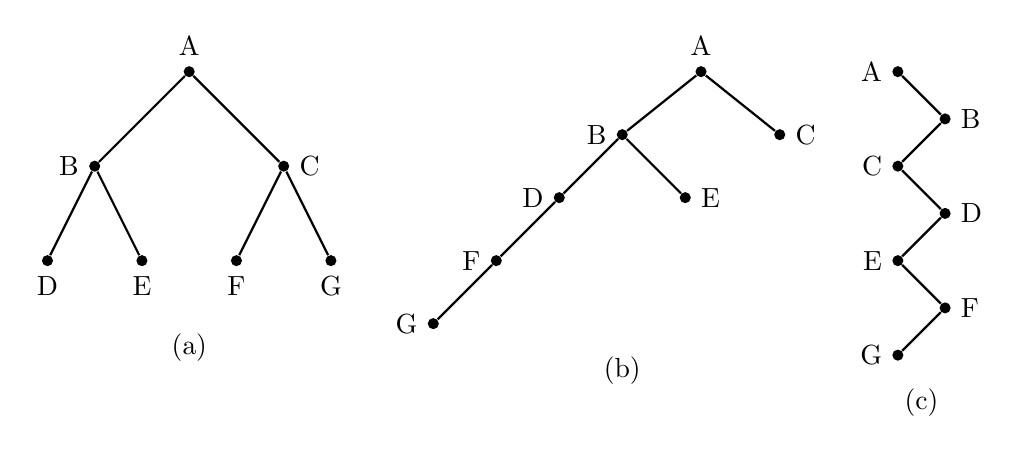
\begin{tikzpicture}[
                dot/.style={circle, fill=black, inner sep=0pt, minimum size=4pt},
                edge/.style={draw, thick},
                label_text/.style={font=\small}
            ]
                % --- CÂY (a) ---
                \begin{scope}[xshift=0cm, yshift=2cm]
                    \node[dot, label=above:A] (A) at (0,0) {};
                    \node[dot, label=left:B] (B) at (-1.2, -1.2) {};
                    \node[dot, label=right:C] (C) at (1.2, -1.2) {};
                    \node[dot, label=below:D] (D) at (-1.8, -2.4) {};
                    \node[dot, label=below:E] (E) at (-0.6, -2.4) {};
                    \node[dot, label=below:F] (F) at (0.6, -2.4) {};
                    \node[dot, label=below:G] (G) at (1.8, -2.4) {};
                    
                    \draw[edge] (A) -- (B); \draw[edge] (A) -- (C);
                    \draw[edge] (B) -- (D); \draw[edge] (B) -- (E);
                    \draw[edge] (C) -- (F); \draw[edge] (C) -- (G);
                    
                    \node at (0, -3.5) {(a)};
                \end{scope}

                % --- CÂY (b) ---
                \begin{scope}[xshift=6.5cm, yshift=2cm]
                    \node[dot, label=above:A] (A) at (0,0) {};
                    \node[dot, label=left:B] (B) at (-1, -0.8) {};
                    \node[dot, label=right:C] (C) at (1, -0.8) {};
                    \node[dot, label=left:D] (D) at (-1.8, -1.6) {};
                    \node[dot, label=right:E] (E) at (-0.2, -1.6) {};
                    \node[dot, label=left:F] (F) at (-2.6, -2.4) {};
                    \node[dot, label=left:G] (G) at (-3.4, -3.2) {};
                    
                    \draw[edge] (A) -- (B); \draw[edge] (A) -- (C);
                    \draw[edge] (B) -- (D); \draw[edge] (B) -- (E);
                    \draw[edge] (D) -- (F);
                    \draw[edge] (F) -- (G);
                    
                    \node at (-1, -3.8) {(b)};
                \end{scope}

                % --- CÂY (c) ---
                \begin{scope}[xshift=9cm, yshift=2cm]
                    \node[dot, label=left:A] (A) at (0,0) {};
                    \node[dot, label=right:B] (B) at (0.6, -0.6) {};
                    \node[dot, label=left:C] (C) at (0, -1.2) {};
                    \node[dot, label=right:D] (D) at (0.6, -1.8) {};
                    \node[dot, label=left:E] (E) at (0, -2.4) {};
                    \node[dot, label=right:F] (F) at (0.6, -3.0) {};
                    \node[dot, label=left:G] (G) at (0, -3.6) {};
                    
                    \draw[edge] (A) -- (B) -- (C) -- (D) -- (E) -- (F) -- (G);
                    
                    \node at (0.3, -4.2) {(c)};
                \end{scope}

            \end{tikzpicture}
            }
        \end{column}
        
        % --- CỘT CÂU HỎI ---
        \begin{column}{0.25\textwidth}
            \small
            1. Cây nào là đầy đủ? \\ \vspace{0.2cm}
            2. Cây nào là hoàn chỉnh? \\ \vspace{0.2cm}
            3. Cây nào là cân đối?
        \end{column}
    \end{columns}
\end{frame}

\section{Cấu trúc dữ liệu biểu diễn cây}
\begin{frame}[t]{1. CẤU TRÚC DỮ LIỆU BIỂU DIỄN CÂY}
    \vspace{0.2cm}
    \begin{itemize}
        % Mục 1.1
        \item \textbf{1.1. Biểu diễn cây bằng mảng}
        \vspace{0.1cm}
        
        % Giả sử T...
        \item Giả sử $T$ là cây với các nút đặt tên là $1, 2, \dots, n$.
        \vspace{0.1cm}
        
        % Biểu diễn T
        \item Biểu diễn $T$:
        \begin{itemize}
            \setlength{\itemsep}{0.2cm} % Tăng khoảng cách giữa các mục con
            
            \item danh sách tuyến tính $A$ trong đó mỗi phần tử $A[i]$ chứa \textcolor{blue}{con trỏ đến cha của nút $i$}.
            
            \item Gốc của $T$ có thể phân biệt bởi con trỏ rỗng.
            
            \item Đặt $A[i] = j$ nếu nút $j$ là cha của nút $i$, \\
            \hspace{0.6cm} $A[i] = 0$ nếu nút $i$ là gốc.
            
            \item thao tác \textbf{parent} trả về cha của một nút
        \end{itemize}
        \vspace{0.2cm}
        
        % Mục cuối cùng
        \item Cách biểu diễn này dựa trên cơ sở là mỗi nút của cây (ngoại trừ gốc) đều có duy nhất một cha.
    \end{itemize}
\end{frame}

\begin{frame}[t]{1. CẤU TRÚC DỮ LIỆU BIỂU DIỄN CÂY}
    \vspace{0.2cm}
    \begin{itemize}
        \item \textbf{1.1. Biểu diễn cây bằng mảng}
        \vspace{0.2cm}
        
        % Ý 1: Thời gian hằng số
        \item Với cách biểu diễn này \textcolor{blue}{cha} của 1 nút có thể xác định trong \textcolor{blue}{thời gian hằng số}.
        \vspace{0.2cm}
        
        % Ý 2: Đường đi
        \item \textcolor{blue}{Đường đi từ 1 nút đến tổ tiên} (kể cả đến gốc) :
        \vspace{0.1cm}
        
        % Công thức
        \begin{center}
            n $\leftarrow$ \textbf{parent}(n) $\leftarrow$ \textbf{parent}(\textbf{parent}(n)) $\leftarrow$ ...
        \end{center}
        \vspace{0.1cm}
        
        % Ý 3: Mảng nhãn
        \item Có thể dùng thêm mảng L[i] để hỗ trợ việc ghi nhận nhãn cho các nút,
        \vspace{0.2cm}
        
        % Ý 4: Bản ghi (Struct)
        \item hoặc biến mỗi phần tử A[i] thành \textcolor{blue}{bản ghi} gồm \textcolor{blue}{2 trường}:
        \begin{itemize}
            \setlength{\itemsep}{0.1cm}
            \item biến nguyên ghi nhận cha
            \item nhãn.
        \end{itemize}
    \end{itemize}
\end{frame}

\begin{frame}[t]{1. CẤU TRÚC DỮ LIỆU BIỂU DIỄN CÂY}
    \vspace{0.2cm}
    \begin{itemize}
        \item \textbf{1.1. Biểu diễn cây bằng mảng}
        \item \textbf{Ví dụ}
    \end{itemize}

    \begin{columns}[T]
        % --- CỘT TRÁI: MẢNG A VÀ TEXT ---
        \begin{column}{0.6\textwidth}
            
            % Vẽ Mảng A
            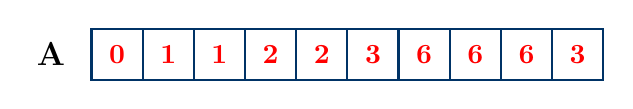
\begin{tikzpicture}
                \node[font=\bfseries\large] at (-0.5, 0.3) {A};
                \foreach \val [count=\i] in {0, 1, 1, 2, 2, 3, 6, 6, 6, 3} {
                    \node[
                        draw=HUSTBlue, 
                        thick, 
                        minimum width=0.65cm, 
                        minimum height=0.65cm, 
                        text=red, 
                        font=\bfseries,
                        anchor=west
                    ] at (\i*0.65 - 0.65, 0.3) {\val};
                }
            \end{tikzpicture}
            \small % Giảm cỡ chữ một chút cho phần liệt kê
    \begin{itemize}
        \setlength{\itemsep}{0.2cm}
        
        \item \textcolor{red}{\textbf{\textit{Hạn chế:}}} Cách dùng con trỏ cha không thích hợp cho các thao tác với con.
        
        \item Cho nút $n$, mất \textcolor{blue}{nhiều thời gian} để xác định các \textcolor{blue}{con của $n$, chiều cao của $n$}.
        
        \item Không cho thứ tự của các nút con $\rightarrow$ \textbf{leftmost\_child} và \textbf{right\_sibling} là không xác định $\rightarrow$ cách biểu diễn này chỉ dùng trong một số trường hợp nhất định.
    \end{itemize}
        \end{column}
        
        % --- CỘT PHẢI: HÌNH CÂY ---
        \begin{column}{0.4\textwidth}
            \centering
            \resizebox{0.95\textwidth}{!}{%
            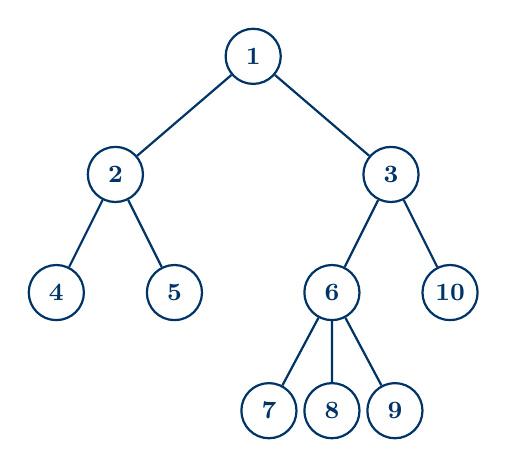
\begin{tikzpicture}[
                level 1/.style={sibling distance=3.5cm, level distance=1.5cm},
                level 2/.style={sibling distance=1.5cm, level distance=1.5cm},
                level 3/.style={sibling distance=0.8cm, level distance=1.5cm},
                treenode/.style={
                    circle, 
                    draw=HUSTBlue, 
                    thick, 
                    text=HUSTBlue, 
                    font=\bfseries\small, 
                    minimum size=0.7cm,
                    inner sep=0pt
                },
                edge from parent/.style={draw=HUSTBlue, thick}
            ]
                % Gốc 1
                \node[treenode] {1}
                    % Con 2
                    child { node[treenode] {2}
                        child { node[treenode] {4} }
                        child { node[treenode] {5} }
                    }
                    % Con 3
                    child { node[treenode] {3}
                        child { node[treenode] {6}
                            child { node[treenode] {7} }
                            child { node[treenode] {8} }
                            child { node[treenode] {9} }
                        }
                        child { node[treenode] {10} }
                    };
            \end{tikzpicture}
            }
        \end{column}
    \end{columns}

    \vspace{0.3cm}
    
\end{frame}

\begin{frame}[t]{1. CẤU TRÚC DỮ LIỆU BIỂU DIỄN CÂY}
    \vspace{0.2cm}
    \begin{itemize}
        \item \textbf{1.2. Biểu diễn cây bằng danh sách các con}
        \vspace{0.3cm}
        
        % Ý 1
        \item Mỗi nút của cây ta cất giữ \textcolor{blue}{1 danh sách các con của nó}.
        \vspace{0.3cm}
        
        % Ý 2
        \item Danh sách con có thể biểu diễn bởi một trong những cách biểu diễn danh sách đã trình bày trong chương trước.
        \vspace{0.3cm}
        
        % Ý 3
        \item \textcolor{blue}{Số lượng con} của các nút là rất \textcolor{blue}{khác nhau} $\rightarrow$ \textcolor{blue}{danh sách móc nối} thường là lựa chọn thích hợp nhất.
    \end{itemize}
\end{frame}

\begin{frame}[t]{1. CẤU TRÚC DỮ LIỆU BIỂU DIỄN CÂY}
    \vspace{0.2cm}
    \begin{itemize}
        \item 1.2. Biểu diễn cây bằng danh sách các con
    \end{itemize}

    \vspace{0.1cm}
    
    \begin{columns}[T]
        % --- CỘT TRÁI: HÌNH CÂY ---
        \begin{column}{0.4\textwidth}
            \centering
            \resizebox{0.95\textwidth}{!}{%
            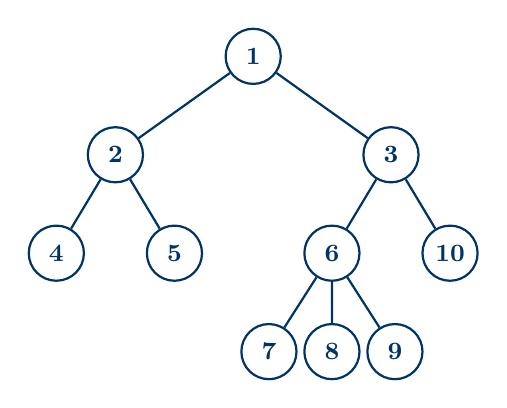
\begin{tikzpicture}[
                level 1/.style={sibling distance=3.5cm, level distance=1.25cm},
                level 2/.style={sibling distance=1.5cm, level distance=1.25cm},
                level 3/.style={sibling distance=0.8cm, level distance=1.25cm},
                % Style nút cây: Tròn, viền xanh, chữ xanh
                treenode/.style={
                    circle, 
                    draw=HUSTBlue, 
                    thick, 
                    text=HUSTBlue, 
                    font=\bfseries\small, 
                    minimum size=0.7cm,
                    inner sep=0pt
                },
                edge from parent/.style={draw=HUSTBlue, thick}
            ]
                % Vẽ cây: 1 -> (2 -> (4,5)), (3 -> (6 -> (7,8,9), 10))
                \node[treenode] {1}
                    child { node[treenode] {2}
                        child { node[treenode] {4} }
                        child { node[treenode] {5} }
                    }
                    child { node[treenode] {3}
                        child { node[treenode] {6}
                            child { node[treenode] {7} }
                            child { node[treenode] {8} }
                            child { node[treenode] {9} }
                        }
                        child { node[treenode] {10} }
                    };
            \end{tikzpicture}
            }
        \end{column}
        
        % --- CỘT PHẢI: CẤU TRÚC DỮ LIỆU ---
        \begin{column}{0.6\textwidth}
            \centering
            \resizebox{0.5\textwidth}{!}{%
            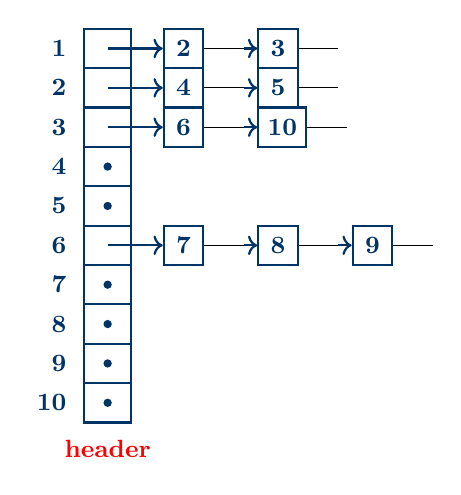
\begin{tikzpicture}[
                % Style cho ô mảng header
                headernode/.style={
                    draw=HUSTBlue, thick,
                    minimum width=0.6cm, minimum height=0.5cm,
                    outer sep=0pt
                },
                % Style cho ô dữ liệu (Linked List Node)
                listnode/.style={
                    draw=HUSTBlue, thick,
                    minimum width=0.5cm, minimum height=0.5cm,
                    font=\bfseries\small\color{HUSTBlue},
                    anchor=west
                },
                % Style cho nhãn chỉ số bên trái
                indexlabel/.style={
                    font=\bfseries\small\color{HUSTBlue},
                    anchor=east
                },
                % Style cho chấm tròn (NULL)
                dot/.style={
                    circle, fill=HUSTBlue, inner sep=0pt, minimum size=3pt
                }
            ]
                % --- 1. Vẽ Mảng Header (10 phần tử) ---
                \foreach \i in {1,...,10} {
                    \node[headernode] (H\i) at (0.3, -\i*0.5) {};
                    \node[indexlabel] at (-0.1, -\i*0.5) {\i};
                }
                \node[text=red, font=\bfseries\small, below=0.1cm] at (H10.south) {header};

                % --- 2. Vẽ các chấm NULL cho các ô trống ---
                \foreach \i in {4, 5, 7, 8, 9, 10} {
                    \node[dot] at (H\i.center) {};
                }

                % --- 3. Vẽ các danh sách liên kết ---
                
                % Dòng 1: -> 2 -> 3
                \node[listnode] (L1_1) at (1.0, -0.5) {2}; \draw (L1_1.east) -- ++(0.5,0); % Ô pointer
                \node[listnode] (L1_2) at (2.2, -0.5) {3}; \draw (L1_2.east) -- ++(0.5,0);
                \draw[->, thick, HUSTBlue] (H1.center) -- (L1_1.west);
                \draw[->, thick, HUSTBlue] (L1_1.east) ++(0.5,0) -- (L1_2.west);
                
                % Dòng 2: -> 4 -> 5
                \node[listnode] (L2_1) at (1.0, -1.0) {4}; \draw (L2_1.east) -- ++(0.5,0);
                \node[listnode] (L2_2) at (2.2, -1.0) {5}; \draw (L2_2.east) -- ++(0.5,0);
                \draw[->, thick, HUSTBlue] (H2.center) -- (L2_1.west);
                \draw[->, thick, HUSTBlue] (L2_1.east) ++(0.5,0) -- (L2_2.west);

                % Dòng 3: -> 6 -> 10
                \node[listnode] (L3_1) at (1.0, -1.5) {6}; \draw (L3_1.east) -- ++(0.5,0);
                \node[listnode] (L3_2) at (2.2, -1.5) {10}; \draw (L3_2.east) -- ++(0.5,0);
                \draw[->, thick, HUSTBlue] (H3.center) -- (L3_1.west);
                \draw[->, thick, HUSTBlue] (L3_1.east) ++(0.5,0) -- (L3_2.west);

                % Dòng 6: -> 7 -> 8 -> 9
                \node[listnode] (L6_1) at (1.0, -3.0) {7}; \draw (L6_1.east) -- ++(0.5,0);
                \node[listnode] (L6_2) at (2.2, -3.0) {8}; \draw (L6_2.east) -- ++(0.5,0);
                \node[listnode] (L6_3) at (3.4, -3.0) {9}; \draw (L6_3.east) -- ++(0.5,0);
                \draw[->, thick, HUSTBlue] (H6.center) -- (L6_1.west);
                \draw[->, thick, HUSTBlue] (L6_1.east) ++(0.5,0) -- (L6_2.west);
                \draw[->, thick, HUSTBlue] (L6_2.east) ++(0.5,0) -- (L6_3.west);

            \end{tikzpicture}
            }
        \end{column}
    \end{columns}

    \vspace{0.1cm}
    \begin{itemize}
        \item Có mảng con trỏ đến đầu các danh sách con của các nút 1, 2, \dots, 10:
    \end{itemize}
    
    \vspace{-0.2cm}
    \hspace{0.5cm} \textcolor{red}{\textit{header}[i] trỏ đến danh sách con của nút $i$.}

\end{frame}

\begin{frame}[t]{1. CẤU TRÚC DỮ LIỆU BIỂU DIỄN CÂY}
    \vspace{0.2cm}
    \begin{itemize}
        \item 1.3. Biểu diễn cây bằng con trái và em kế cận phải
    \end{itemize}

    \vspace{0.2cm}
    
    \begin{columns}[T]
        % --- CỘT TRÁI: NHẬN XÉT ---
        \begin{column}{0.48\textwidth}
            % Tạo khung viền xanh, nền trắng
            \setlength{\fboxrule}{0.8pt} % Độ dày viền
            \fcolorbox{HUSTBlue}{white}{%
                \begin{minipage}{0.95\textwidth}
                    \vspace{0.1cm}
                    \textbf{Nhận xét:}
                    \begin{itemize}
                        \item Mỗi một nút của cây hoặc là
                        \begin{itemize}
                            \item không có con
                            \item có đúng 1 nút con cực trái
                            \item không có em kế cận phải
                            \item có đúng 1 nút em kế cận phải
                        \end{itemize}
                    \end{itemize}
                    
                    \vspace{0.1cm}
                    $\rightarrow$ Để biểu diễn cây: lưu trữ thông tin về con cực trái và em kế cận phải của mỗi nút.
                    \vspace{0.1cm}
                \end{minipage}
            }
        \end{column}
        
        % --- CỘT PHẢI: MÃ CODE ---
        \begin{column}{0.5\textwidth}
            % Tạo khung viền xanh, nền trắng
            \setlength{\fboxrule}{0.8pt}
            \fcolorbox{HUSTBlue}{white}{%
                \begin{minipage}{0.95\textwidth}
                    \vspace{0.1cm}
                    \textbf{Sử dụng mô tả sau:}
                    \vspace{0.3cm}
                    
                    % Code giả lập (Manual coloring để giống hệt hình)
                    \ttfamily\small
                    \textcolor{red}{struct} \textcolor{red}{Tnode} \\
                    \{ \\
                    \hspace*{0.4cm} \textcolor{red}{char} word[20]; \textcolor{violet}{// Dữ liệu cất giữ ở nút} \\
                    \hspace*{0.4cm} \textcolor{red}{struct} \textcolor{red}{Tnode} *leftmost\_child; \\
                    \hspace*{0.4cm} \textcolor{red}{struct} \textcolor{red}{Tnode} *right\_sibling; \\
                    \}; \\
                    \textcolor{red}{typedef} \textcolor{red}{struct} \textcolor{red}{Tnode} \textcolor{red}{treeNode}; \\
                    \textcolor{red}{treeNode} Root;
                    
                    \vspace{0.1cm}
                \end{minipage}
            }
        \end{column}
    \end{columns}
\end{frame}

\begin{frame}[fragile, t]{1. CẤU TRÚC DỮ LIỆU BIỂU DIỄN CÂY}
    \vspace{0.2cm}
    \begin{itemize}
        \item 1.3. Biểu diễn cây bằng con trái và em kế cận phải
    \end{itemize}

    \vspace{0.2cm}
    
    \begin{columns}[T]
        % --- CỘT TRÁI: CÂY TỔNG QUÁT ---
        \begin{column}{0.4\textwidth}
            \centering
            \resizebox{0.95\textwidth}{!}{%
            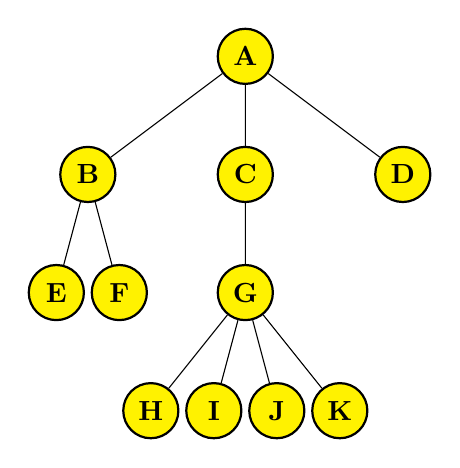
\begin{tikzpicture}[
                level 1/.style={sibling distance=2.0cm, level distance=1.5cm},
                level 2/.style={sibling distance=0.8cm, level distance=1.5cm},
                level 3/.style={sibling distance=0.8cm, level distance=1.5cm},
                treenode/.style={
                    circle, 
                    draw=black, 
                    fill=yellow, 
                    thick, 
                    font=\bfseries, 
                    minimum size=0.7cm,
                    inner sep=0pt
                },
                edge from parent/.style={draw=black, thin}
            ]
                \node[treenode] {A}
                    child { node[treenode] {B}
                        child { node[treenode] {E} }
                        child { node[treenode] {F} }
                    }
                    child { node[treenode] {C}
                        child { node[treenode] {G}
                            child { node[treenode] {H} }
                            child { node[treenode] {I} }
                            child { node[treenode] {J} }
                            child { node[treenode] {K} }
                        }
                    }
                    child { node[treenode] {D} };
            \end{tikzpicture}
            }
            \vspace{0.2cm}
            \par \textbf{Cây tổng quát}
        \end{column}
        
        % --- CỘT PHẢI: BIỂU DIỄN CÂY ---
        \begin{column}{0.6\textwidth}
            \centering
            \resizebox{0.95\textwidth}{!}{%
            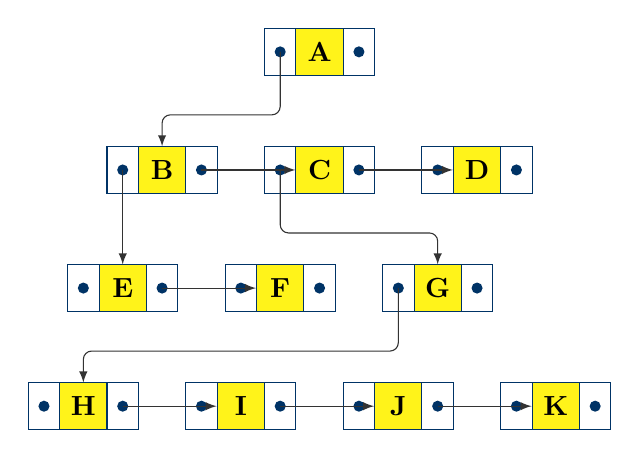
\begin{tikzpicture}[
                % Định nghĩa hình dáng node cấu trúc dữ liệu
                dsnode/.pic={
                    \node[draw=HUSTBlue, fill=white, minimum width=0.4cm, minimum height=0.6cm] (-l) at (-0.5,0) {};
                    \fill[HUSTBlue] (-l.center) circle (2pt);
                    \node[draw=HUSTBlue, fill=yellow!90, minimum width=0.6cm, minimum height=0.6cm, font=\bfseries] (-d) at (0,0) {#1};
                    \node[draw=HUSTBlue, fill=white, minimum width=0.4cm, minimum height=0.6cm] (-r) at (0.5,0) {};
                    \fill[HUSTBlue] (-r.center) circle (2pt);
                    \coordinate (-top) at (0, 0.3);
                },
                node distance=1.5cm and 0.5cm,
                arrow/.style={->, >=latex, draw=black!80, thin, rounded corners=3pt}
            ]
                % Row 1
                \path (2, 0) pic (A) {dsnode=A};
                % Row 2
                \path (0, -1.5) pic (B) {dsnode=B};
                \path (2, -1.5) pic (C) {dsnode=C};
                \path (4, -1.5) pic (D) {dsnode=D};
                % Row 3
                \path (-0.5, -3) pic (E) {dsnode=E};
                \path (1.5, -3) pic (F) {dsnode=F};
                \path (3.5, -3) pic (G) {dsnode=G};
                % Row 4
                \path (-1, -4.5) pic (H) {dsnode=H};
                \path (1, -4.5) pic (I) {dsnode=I};
                \path (3, -4.5) pic (J) {dsnode=J};
                \path (5, -4.5) pic (K) {dsnode=K};

                % Connectors
                \draw[arrow] (A-l.center) -- ++(0,-0.8) -| (B-top);
                \draw[arrow] (B-r.center) -- (C-d.west);
                \draw[arrow] (C-r.center) -- (D-d.west);
                \draw[arrow] (B-l.center) -- ++(0,-0.8) -| (E-top);
                \draw[arrow] (E-r.center) -- (F-d.west);
                \draw[arrow] (C-l.center) -- ++(0,-0.8) -| (G-top);
                \draw[arrow] (G-l.center) -- ++(0,-0.8) -| (H-top);
                \draw[arrow] (H-r.center) -- (I-d.west);
                \draw[arrow] (I-r.center) -- (J-d.west);
                \draw[arrow] (J-r.center) -- (K-d.west);

            \end{tikzpicture}
            }
            \vspace{0.2cm}
            \par \textbf{Biểu diễn cây}
        \end{column}
    \end{columns}
\end{frame}

\begin{frame}[t]{1. CẤU TRÚC DỮ LIỆU BIỂU DIỄN CÂY}
    \vspace{0.2cm}
    \begin{itemize}
        \item 1.3. Biểu diễn cây bằng con trái và em kế cận phải
    \end{itemize}

    \vspace{0.2cm}
    \textbf{Nhận xét:}
    \vspace{0.1cm}

    \begin{itemize}
        \setlength{\itemsep}{0.4cm} % Tăng khoảng cách giữa các ý chính
        
        \item Với cách biểu diễn này, các thao tác cơ bản dễ dàng cài đặt.
        
        \item Chỉ có thao tác \textbf{parent} là đòi hỏi phải duyệt danh sách nên không hiệu quả.
        
        \begin{itemize}
            \vspace{0.1cm} % Khoảng cách nhỏ cho ý phụ
            \item Trong trường hợp phép toán này phải dùng thường xuyên, bổ sung thêm một trường nữa vào bản ghi để lưu cha của nút.
        \end{itemize}
    \end{itemize}
\end{frame}
\section{Duyệt cây}
\begin{frame}[t]{2. DUYỆT CÂY}
    \vspace{0.2cm}
    \begin{itemize}
        \setlength{\itemsep}{0.3cm} % Tăng khoảng cách giữa các mục chính
        
        \item Xếp thứ tự các nút
        \begin{itemize}
            \item \textbf{Thứ tự trước, Thứ tự sau và Thứ tự giữa (Preorder, Postorder và Inorder)}
        \end{itemize}
        
        \item Các thứ tự này được định nghĩa một cách đệ qui như sau
        \begin{itemize}
            \setlength{\itemsep}{0.2cm} % Khoảng cách giữa các định nghĩa
            
            \item \textcolor{blue}{Nếu cây $T$ là rỗng}, thì danh sách rỗng là danh sách theo thứ tự trước, thứ tự sau và thứ tự giữa của cây $T$.
            
            \item \textcolor{blue}{Nếu cây $T$ có 1 nút}, thì nút đó chính là danh sách theo thứ tự trước, thứ tự sau và thứ tự giữa của cây $T$.
            
            \item \textcolor{blue}{Trái lại}, giả sử $T$ là cây có gốc $r$ với các cây con là $T_1, T_2, \dots, T_k$.
        \end{itemize}
    \end{itemize}
\end{frame}

\begin{frame}[t]{2. DUYỆT CÂY}
    \vspace{0.2cm}
    \begin{itemize}
        \item \textbf{2.1. Duyệt theo thứ tự trước}
    \end{itemize}

    \vspace{0.1cm}
    \centering
    
    % Resize hình vẽ vừa phải (khoảng 60% chiều rộng)
    \resizebox{0.35\textwidth}{!}{%
    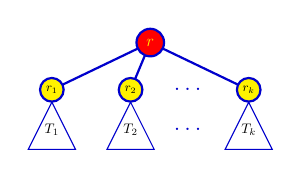
\begin{tikzpicture}[
        scale=0.5, transform shape,
        % Style cho nút gốc: Đỏ, chữ vàng
        rootnode/.style={
            circle, 
            draw=blue!80!black, 
            fill=red, 
            text=yellow, 
            thick, 
            minimum size=0.7cm, 
            inner sep=0pt, 
            font=\bfseries\large
        },
        % Style cho nút con: Vàng, chữ đen
        childnode/.style={
            circle, 
            draw=blue!80!black, 
            fill=yellow, 
            text=black, 
            thick, 
            minimum size=0.6cm, 
            inner sep=0pt, 
            font=\small\bfseries
        },
        % Style tam giác cây con
        subtree/.style={
            draw=blue!80!black, 
            thin
        },
        % Style cạnh nối
        edge/.style={
            draw=blue!80!black, 
            thick
        }
    ]

        % --- VẼ CÁC NÚT ---
        % Root
        \node[rootnode] (r) at (0,0) {$r$};

        % Children (cách nhau đều)
        \node[childnode] (r1) at (-2.5, -1.2) {$r_1$};
        \node[childnode] (r2) at (-0.5, -1.2) {$r_2$};
        
        % Dấu ... giữa các con
        \node[font=\bfseries\LARGE\color{blue!80!black}] at (1.0, -1.2) {$\dots$};
        
        \node[childnode] (rk) at (2.5, -1.2) {$r_k$};

        % --- VẼ CẠNH ---
        \draw[edge] (r) -- (r1);
        \draw[edge] (r) -- (r2);
        \draw[edge] (r) -- (rk);

        % --- VẼ TAM GIÁC CÂY CON ---
        % T1
        \draw[subtree] (r1.south) -- ++(-0.6, -1.2) -- ++(1.2, 0) -- cycle;
        \node at ($(r1.south) + (0, -0.7)$) {$T_1$};

        % T2
        \draw[subtree] (r2.south) -- ++(-0.6, -1.2) -- ++(1.2, 0) -- cycle;
        \node at ($(r2.south) + (0, -0.7)$) {$T_2$};
        
        % Dấu ... dưới đáy
        \node[font=\bfseries\LARGE\color{blue!80!black}] at (1.0, -2.2) {$\dots$};

        % Tk
        \draw[subtree] (rk.south) -- ++(-0.6, -1.2) -- ++(1.2, 0) -- cycle;
        \node at ($(rk.south) + (0, -0.7)$) {$T_k$};

    \end{tikzpicture}
    }

    \vspace{0.1cm}
    \begin{itemize}
        \item \textbf{Thứ tự trước} (hay duyệt theo thứ tự trước - \textit{preorder traversal}) của các nút của $T$ là:
        \begin{itemize}
            \setlength{\itemsep}{0.1cm}
            \item Gốc $r$ của $T$,
            \item Tiếp đến là các nút của $T_1$ theo thứ tự trước,
            \item Tiếp đến là các nút của $T_2$ theo thứ tự trước,
            \item ...
            \item Và cuối cùng là các nút của $T_k$ theo thứ tự trước.
        \end{itemize}
    \end{itemize}
\end{frame}

\begin{frame}[t]{2. DUYỆT CÂY}
    \vspace{0.2cm}
    \begin{itemize}
        \item \textbf{2.1. Duyệt theo thứ tự trước}
    \end{itemize}
    
    Thuật toán:
    \vspace{0.2cm}

    \begin{columns}[T]
        % --- CỘT TRÁI: MÃ GIẢ & KẾT QUẢ ---
        \begin{column}{0.65\textwidth}
            % Mã giả
            \small
            \textbf{void} PREORDER ( $nodeT \ r$ ) \\
            \{ \\
            (1) \hspace{0.2cm} Đưa ra $r$; \\
            (2) \hspace{0.2cm} \textbf{for} (mỗi con $c$ của $r$, nếu có, theo thứ tự từ trái sang) \textbf{do} \\
            \hspace{1.5cm} PREORDER($c$); \\
            \}
            
            \vspace{0.6cm}
            \textbf{Ví dụ:} Thứ tự trước của các đỉnh của cây trên hình vẽ là
            \vspace{0.2cm}
            
            \centering
            \textbf{\textit{a, b, c, e, h, i, f, j, d, g}}
        \end{column}
        
        % --- CỘT PHẢI: CÂY MINH HỌA ---
        \begin{column}{0.4\textwidth}
            \centering
            \resizebox{0.95\textwidth}{!}{%
            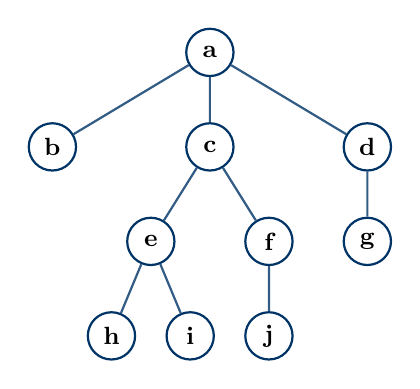
\begin{tikzpicture}[
                level 1/.style={sibling distance=2.0cm, level distance=1.2cm},
                level 2/.style={sibling distance=1.5cm, level distance=1.2cm},
                level 3/.style={sibling distance=1.0cm, level distance=1.2cm},
                % Style cho nút: Tròn, viền xanh, chữ đen
                treenode/.style={
                    circle, 
                    draw=HUSTBlue, 
                    thick, 
                    text=black, 
                    font=\bfseries\small, 
                    minimum size=0.6cm,
                    inner sep=0pt
                },
                % Style cạnh: Màu xanh nhạt hơn chút
                edge from parent/.style={
                    draw=HUSTBlue!80, 
                    thick
                }
            ]
                % Cấu trúc cây: a -> (b, c(e(h,i), f(j)), d(g))
                \node[treenode] {a}
                    % Nhánh b
                    child { node[treenode] {b} }
                    % Nhánh c
                    child { node[treenode] {c}
                        child { node[treenode] {e}
                            child { node[treenode] {h} }
                            child { node[treenode] {i} }
                        }
                        child { node[treenode] {f}
                            child { node[treenode] {j} }
                        }
                    }
                    % Nhánh d
                    child { node[treenode] {d}
                        child { node[treenode] {g} }
                    };
            \end{tikzpicture}
            }
        \end{column}
    \end{columns}
\end{frame}

\begin{frame}[t]{2. DUYỆT CÂY}
    \vspace{0.2cm}
    \begin{itemize}
        \item \textbf{2.1. Duyệt theo thứ tự sau}
    \end{itemize}

    \vspace{0.1cm}
    \centering
    
    % Resize hình vẽ vừa phải (khoảng 60% chiều rộng)
    \resizebox{0.35\textwidth}{!}{%
    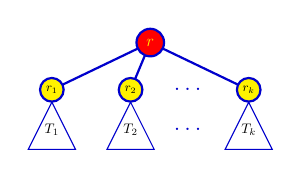
\begin{tikzpicture}[
        scale=0.5, transform shape,
        % Style cho nút gốc: Đỏ, chữ vàng
        rootnode/.style={
            circle, 
            draw=blue!80!black, 
            fill=red, 
            text=yellow, 
            thick, 
            minimum size=0.7cm, 
            inner sep=0pt, 
            font=\bfseries\large
        },
        % Style cho nút con: Vàng, chữ đen
        childnode/.style={
            circle, 
            draw=blue!80!black, 
            fill=yellow, 
            text=black, 
            thick, 
            minimum size=0.6cm, 
            inner sep=0pt, 
            font=\small\bfseries
        },
        % Style tam giác cây con
        subtree/.style={
            draw=blue!80!black, 
            thin
        },
        % Style cạnh nối
        edge/.style={
            draw=blue!80!black, 
            thick
        }
    ]

        % --- VẼ CÁC NÚT ---
        % Root
        \node[rootnode] (r) at (0,0) {$r$};

        % Children (cách nhau đều)
        \node[childnode] (r1) at (-2.5, -1.2) {$r_1$};
        \node[childnode] (r2) at (-0.5, -1.2) {$r_2$};
        
        % Dấu ... giữa các con
        \node[font=\bfseries\LARGE\color{blue!80!black}] at (1.0, -1.2) {$\dots$};
        
        \node[childnode] (rk) at (2.5, -1.2) {$r_k$};

        % --- VẼ CẠNH ---
        \draw[edge] (r) -- (r1);
        \draw[edge] (r) -- (r2);
        \draw[edge] (r) -- (rk);

        % --- VẼ TAM GIÁC CÂY CON ---
        % T1
        \draw[subtree] (r1.south) -- ++(-0.6, -1.2) -- ++(1.2, 0) -- cycle;
        \node at ($(r1.south) + (0, -0.7)$) {$T_1$};

        % T2
        \draw[subtree] (r2.south) -- ++(-0.6, -1.2) -- ++(1.2, 0) -- cycle;
        \node at ($(r2.south) + (0, -0.7)$) {$T_2$};
        
        % Dấu ... dưới đáy
        \node[font=\bfseries\LARGE\color{blue!80!black}] at (1.0, -2.2) {$\dots$};

        % Tk
        \draw[subtree] (rk.south) -- ++(-0.6, -1.2) -- ++(1.2, 0) -- cycle;
        \node at ($(rk.south) + (0, -0.7)$) {$T_k$};

    \end{tikzpicture}
    }

    \vspace{0.1cm}
    \begin{itemize}
        \item \textbf{Thứ tự sau} của các nút của cây $T$ là:
        \begin{itemize}
            \setlength{\itemsep}{0.1cm}
            \item Các nút của $T_1$
theo thứ tự sau,
            \item tiếp đến là các nút của $T_2$
theo thứ tự sau,
            \item ...
            \item các nút của $T_k$ theo thứ tự sau,
            \item sau cùng là nút gốc $r$.
        \end{itemize}
    \end{itemize}
\end{frame}

\begin{frame}[t]{2. DUYỆT CÂY}
    \vspace{0.2cm}
    \begin{itemize}
        \item \textbf{2.1. Duyệt theo thứ tự sau}
    \end{itemize}
    
    Thuật toán:

    \begin{columns}[T]
        % --- CỘT TRÁI: MÃ GIẢ & KẾT QUẢ ---
        \begin{column}{0.65\textwidth}
            % Mã giả
            \small
            \textbf{void} POSTORDER( $nodeT \ r$ ) \\
            \{ \\
            \textbf{for} (mỗi con $c$ của $r$, nếu có, theo thứ tự từ trái sang) \textbf{do}
            \hspace{1.5cm} POSTORDER($c$); \\
            Đưa ra $r$;\\
            \}
            
            \vspace{0.4cm}
            \textbf{Ví dụ:} Dãy các đỉnh được liệt kê theo \textbf{thứ tự sau} của cây
trong hình vẽ là:
            \vspace{0.2cm}
            
            \centering
            \textbf{\textit{b, h, i, e, j, f, c, g, d, a}}
        \end{column}
        
        % --- CỘT PHẢI: CÂY MINH HỌA ---
        \begin{column}{0.4\textwidth}
            \centering
            \resizebox{0.95\textwidth}{!}{%
            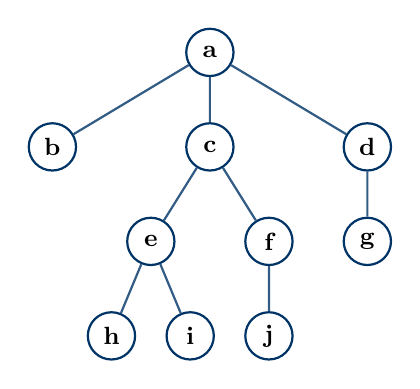
\begin{tikzpicture}[
                level 1/.style={sibling distance=2.0cm, level distance=1.2cm},
                level 2/.style={sibling distance=1.5cm, level distance=1.2cm},
                level 3/.style={sibling distance=1.0cm, level distance=1.2cm},
                % Style cho nút: Tròn, viền xanh, chữ đen
                treenode/.style={
                    circle, 
                    draw=HUSTBlue, 
                    thick, 
                    text=black, 
                    font=\bfseries\small, 
                    minimum size=0.6cm,
                    inner sep=0pt
                },
                % Style cạnh: Màu xanh nhạt hơn chút
                edge from parent/.style={
                    draw=HUSTBlue!80, 
                    thick
                }
            ]
                % Cấu trúc cây: a -> (b, c(e(h,i), f(j)), d(g))
                \node[treenode] {a}
                    % Nhánh b
                    child { node[treenode] {b} }
                    % Nhánh c
                    child { node[treenode] {c}
                        child { node[treenode] {e}
                            child { node[treenode] {h} }
                            child { node[treenode] {i} }
                        }
                        child { node[treenode] {f}
                            child { node[treenode] {j} }
                        }
                    }
                    % Nhánh d
                    child { node[treenode] {d}
                        child { node[treenode] {g} }
                    };
            \end{tikzpicture}
            }
        \end{column}
    \end{columns}
\end{frame}

\begin{frame}[t]{2. DUYỆT CÂY}
    \vspace{0.2cm}
    \begin{itemize}
        \item \textbf{2.1. Duyệt theo thứ tự sau}
    \end{itemize}

    \vspace{0.1cm}
    \centering
    
    % Resize hình vẽ vừa phải (khoảng 60% chiều rộng)
    \resizebox{0.35\textwidth}{!}{%
    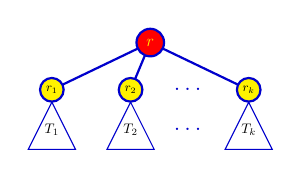
\begin{tikzpicture}[
        scale=0.5, transform shape,
        % Style cho nút gốc: Đỏ, chữ vàng
        rootnode/.style={
            circle, 
            draw=blue!80!black, 
            fill=red, 
            text=yellow, 
            thick, 
            minimum size=0.7cm, 
            inner sep=0pt, 
            font=\bfseries\large
        },
        % Style cho nút con: Vàng, chữ đen
        childnode/.style={
            circle, 
            draw=blue!80!black, 
            fill=yellow, 
            text=black, 
            thick, 
            minimum size=0.6cm, 
            inner sep=0pt, 
            font=\small\bfseries
        },
        % Style tam giác cây con
        subtree/.style={
            draw=blue!80!black, 
            thin
        },
        % Style cạnh nối
        edge/.style={
            draw=blue!80!black, 
            thick
        }
    ]

        % --- VẼ CÁC NÚT ---
        % Root
        \node[rootnode] (r) at (0,0) {$r$};

        % Children (cách nhau đều)
        \node[childnode] (r1) at (-2.5, -1.2) {$r_1$};
        \node[childnode] (r2) at (-0.5, -1.2) {$r_2$};
        
        % Dấu ... giữa các con
        \node[font=\bfseries\LARGE\color{blue!80!black}] at (1.0, -1.2) {$\dots$};
        
        \node[childnode] (rk) at (2.5, -1.2) {$r_k$};

        % --- VẼ CẠNH ---
        \draw[edge] (r) -- (r1);
        \draw[edge] (r) -- (r2);
        \draw[edge] (r) -- (rk);

        % --- VẼ TAM GIÁC CÂY CON ---
        % T1
        \draw[subtree] (r1.south) -- ++(-0.6, -1.2) -- ++(1.2, 0) -- cycle;
        \node at ($(r1.south) + (0, -0.7)$) {$T_1$};

        % T2
        \draw[subtree] (r2.south) -- ++(-0.6, -1.2) -- ++(1.2, 0) -- cycle;
        \node at ($(r2.south) + (0, -0.7)$) {$T_2$};
        
        % Dấu ... dưới đáy
        \node[font=\bfseries\LARGE\color{blue!80!black}] at (1.0, -2.2) {$\dots$};

        % Tk
        \draw[subtree] (rk.south) -- ++(-0.6, -1.2) -- ++(1.2, 0) -- cycle;
        \node at ($(rk.south) + (0, -0.7)$) {$T_k$};

    \end{tikzpicture}
    }

    \vspace{0.1cm}
    \begin{itemize}
        \item \textbf{Thứ tự giữa} của các nút của cây $T$ là:
        \begin{itemize}
            \setlength{\itemsep}{0.1cm}
            \item Các nút của $T_1$
theo thứ tự giữa,
            \item tiếp đến là nút gốc $r$,
            \item Tiếp theo là các nút của $T_2$,...,$T_k$, mỗi nhóm nút được xếp theo thứ tự giữa.
        \end{itemize}
    \end{itemize}
\end{frame}

\begin{frame}[t]{2. DUYỆT CÂY}
    \begin{itemize}
        \item \textbf{2.3. Duyệt theo thứ tự giữa}
    \end{itemize}
    
    \begin{columns}[T]
        % --- CỘT TRÁI: THUẬT TOÁN & VÍ DỤ ---
        \begin{column}{0.65\textwidth}
            \small
            \textbf{void} INORDER ( $nodeT \ r$ ) \\
            \{ \\
            % Tô nền xanh nhạt cho dòng if
            \hspace{0.3cm} \colorbox{blue!10}{\textbf{if} ( $r$ là lá ) Đưa ra $r$;} \\
            \hspace{0.3cm} \textbf{else} \\
            \hspace{0.3cm} \{ \\
            \hspace{1.0cm} INORDER(con trái nhất của $r$); \\
            \hspace{1.0cm} Đưa ra $r$; \\
            \hspace{1.0cm} \textbf{for} (mỗi con $c$ của $r$, ngoại trừ con trái nhất, theo thứ tự từ trái sang) \textbf{do} \\
            \hspace{2.0cm} INORDER($c$); \\
            \hspace{0.3cm} \} \\
            \}
        \end{column}
        
        % --- CỘT PHẢI: HÌNH CÂY ---
        \begin{column}{0.35\textwidth}
            \centering
            \resizebox{0.95\textwidth}{!}{%
            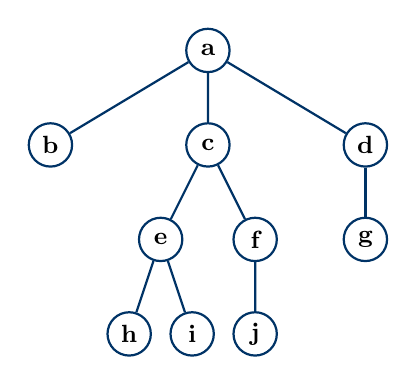
\begin{tikzpicture}[
                level 1/.style={sibling distance=2.0cm, level distance=1.2cm},
                level 2/.style={sibling distance=1.2cm, level distance=1.2cm},
                level 3/.style={sibling distance=0.8cm, level distance=1.2cm},
                % Style nút: Tròn, viền xanh, chữ đen
                treenode/.style={
                    circle, 
                    draw=HUSTBlue, 
                    thick, 
                    text=black, 
                    font=\bfseries\small, 
                    minimum size=0.55cm,
                    inner sep=1pt
                },
                edge from parent/.style={draw=HUSTBlue, thick}
            ]
                % Vẽ cây: a -> (b, c(e(h,i), f(j)), d(g))
                % Lưu ý: Cấu trúc cây này khớp với kết quả duyệt: b, a, ... g, d
                \node[treenode] {a}
                    child { node[treenode] {b} }
                    child { node[treenode] {c}
                        child { node[treenode] {e}
                            child { node[treenode] {h} }
                            child { node[treenode] {i} }
                        }
                        child { node[treenode] {f}
                            child { node[treenode] {j} }
                        }
                    }
                    child { node[treenode] {d}
                        child { node[treenode] {g} }
                    };
            \end{tikzpicture}
            }
        \end{column}
    \end{columns}
    \begin{itemize}
                \item \textbf{Ví dụ:} Dãy các đỉnh của cây trong hình vẽ được liệt kê theo thứ tự giữa:
            \end{itemize}
            \vspace{-0.1cm}
            \centering
            \textbf{\textit{b, a, h, e, i, c, j, f, g, d}}
\end{frame}

\begin{frame}[t]{2. DUYỆT CÂY}
    \begin{itemize}
        \item Xếp thứ tự các nút
    \end{itemize}

    
    \begin{columns}[T]
        % --- CỘT TRÁI: TEXT MÔ TẢ ---
        \begin{column}{0.55\textwidth}
            \vspace{0.2cm}
            \large
            Đi vòng quanh bên ngoài cây bắt đầu từ gốc, ngược chiều kim đồn g hồ và sát theo cây nhất
        \end{column}
        
        % --- CỘT PHẢI: HÌNH MINH HỌA ---
        \begin{column}{0.45\textwidth}
            \centering
            \resizebox{0.65\textwidth}{!}{%
            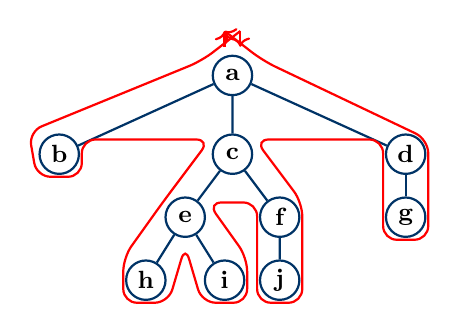
\begin{tikzpicture}[
                level 1/.style={sibling distance=2.2cm, level distance=1.0cm},
                level 2/.style={sibling distance=1.2cm, level distance=0.8cm},
                level 3/.style={sibling distance=1.0cm, level distance=0.8cm},
                % Style nút: Tròn, trắng, viền xanh
                treenode/.style={
                    circle, 
                    draw=HUSTBlue, 
                    thick, 
                    fill=white,
                    text=black, 
                    font=\bfseries\small, 
                    minimum size=0.5cm,
                    inner sep=1pt
                },
                edge from parent/.style={draw=HUSTBlue, thick}
            ]
                % 1. VẼ CÂY
                \node[treenode] (a) {a}
                    child { node[treenode] (b) {b} }
                    child { node[treenode] (c) {c}
                        child { node[treenode] (e) {e}
                            child { node[treenode] (h) {h} }
                            child { node[treenode] (i) {i} }
                        }
                        child { node[treenode] (f) {f}
                            child { node[treenode] (j) {j} }
                        }
                    }
                    child { node[treenode] (d) {d}
                        child { node[treenode] (g) {g} }
                    };

                % 2. VẼ ĐƯỜNG BAO QUANH (CONTOUR) MÀU ĐỎ
                % Sử dụng tọa độ tương đối và rounded corners để tạo đường cong mềm
                \draw[red, thick, rounded corners=5pt, ->] 
                    ($(a.north)+(0.1, 0.3)$) -- 
                    ($(a.north west)+(-0.2, 0)$) -- 
                    ($(b.north west)+(-0.2, 0.1)$) -- 
                    ($(b.south west)+(-0.1, -0.1)$) -- 
                    ($(b.south east)+(0.1, -0.1)$) -- 
                    ($(b.north east)+(0.1, 0)$) -- 
                    ($(c.north west)+(-0.1, 0)$) -- 
                    ($(e.north west)+(-0.1, 0)$) -- 
                    ($(h.north west)+(-0.1, 0.1)$) -- 
                    ($(h.south west)+(-0.1, -0.1)$) -- 
                    ($(h.south east)+(0.1, -0.1)$) -- 
                    ($(e.south)+(0, -0.1)$) -- % Giữa h và i
                    ($(i.south west)+(-0.1, -0.1)$) -- 
                    ($(i.south east)+(0.1, -0.1)$) -- 
                    ($(i.north east)+(0.1, 0.1)$) -- 
                    ($(e.north east)+(0.1, 0)$) -- 
                    ($(f.north west)+(-0.1, 0)$) -- 
                    ($(j.north west)+(-0.1, 0.1)$) -- 
                    ($(j.south west)+(-0.1, -0.1)$) -- 
                    ($(j.south east)+(0.1, -0.1)$) -- 
                    ($(j.north east)+(0.1, 0.1)$) -- 
                    ($(f.north east)+(0.1, 0)$) -- 
                    ($(c.north east)+(0.1, 0)$) -- 
                    ($(d.north west)+(-0.1, 0)$) -- % Notch giữa c và d
                    ($(g.south west)+(-0.1, -0.1)$) -- % Bao quanh g (con của d)
                    ($(g.south east)+(0.1, -0.1)$) -- 
                    ($(d.north east)+(0.1, 0)$) -- 
                    ($(a.north east)+(0.2, 0)$) -- 
                    ($(a.north)+(-0.1, 0.3)$);

                % Mũi tên chỉ hướng bắt đầu/kết thúc
                \draw[red, ->, thick] ($(a.north)+(0.1, 0.3)$) -- ($(a.north)+(0.1, 0.1)$);
                \draw[red, ->, thick] ($(a.north)+(-0.1, 0.1)$) -- ($(a.north)+(-0.1, 0.3)$);

            \end{tikzpicture}
            }
        \end{column}
    \end{columns}
    
    % --- KHUNG TEXT ---
    % Sử dụng fcolorbox để tạo khung viền xanh
    \setlength{\fboxrule}{0.8pt}
    \fcolorbox{HUSTBlue}{white}{%
        \begin{minipage}{0.96\textwidth}
            \vspace{0.1cm}
            \small
            \begin{itemize}
                \setlength{\itemsep}{0.2cm}
                
                \item \textcolor{red}{Thứ tự trước:} đưa ra nút mỗi khi đi qua nó.
                
                \item \textcolor{red}{Thứ tự sau:} đưa ra nút khi qua nó ở lần cuối trước khi quay về cha của nó.
                
                \item \textcolor{red}{Thứ tự giữa:} đưa ra lá ngay khi đi qua nó, còn những nút trong được đưa ra khi lần thứ hai được đi qua.
                
                \item \textbf{\textcolor{HUSTBlue}{Chú ý:}} các lá được xếp thứ tự từ trái sang phải như nhau trong cả 3 cách sắp xếp.
            \end{itemize}
            \vspace{0.1cm}
        \end{minipage}
    }
\end{frame}
\section{Cây nhị phân}
\begin{frame}[t]{3. CÂY NHỊ PHÂN}
    \vspace{0.2cm}
    \begin{itemize}
        \item \textbf{3.1. Biểu diễn cây nhị phân}
        
        \begin{itemize}
            \item \textbf{Biểu diễn sử dụng mảng}
            \vspace{0.3cm}
            
            \item Tương tự như trong cách biểu diễn cây tổng quát.
            \vspace{0.3cm}
            
            \item Trong trường hợp cây nhị phân hoàn chỉnh, có thể cài đặt nhiều phép toán với cây rất hiệu quả.
            \vspace{0.2cm}
            
            \begin{itemize}
                \setlength{\itemsep}{0.3cm} % Tăng khoảng cách giữa các ý nhỏ
                
                \item Xét cây nhị phân hoàn chỉnh $T$ có $n$ nút, trong đó mỗi nút chứa một giá trị.
                
                \item Gán tên cho các nút của cây nhị phân hoàn chỉnh $T$ từ trên xuống dưới và từ trái qua phải bằng các số $1, 2, \dots, n$.
                
                \item Đặt tương ứng cây $T$ với \textcolor{red}{\textbf{mảng A}} trong đó phần tử thứ $i$ của A là giá trị cất giữ trong nút thứ $i$ của cây $T$, $i = 1, 2, \dots, n$.
            \end{itemize}
        \end{itemize}
    \end{itemize}
\end{frame}

\begin{frame}[t]{3. CÂY NHỊ PHÂN}
    \begin{itemize}
        \item \textbf{3.1. Biểu diễn cây nhị phân}
        \begin{itemize}
            \item \textbf{Biểu diễn sử dụng mảng}
        \end{itemize}
    \end{itemize}
    \centering
    
    % Resize toàn bộ hình vẽ cho vừa slide
    \resizebox{0.67\textwidth}{!}{%
    \begin{tikzpicture}[
        % Cấu hình cây
        level 1/.style={sibling distance=6cm, level distance=1.8cm},
        level 2/.style={sibling distance=3cm, level distance=1.8cm},
        level 3/.style={sibling distance=1.5cm, level distance=1.8cm},
        % Style nút cây: Tròn, nền xanh sáng (cyan), chữ trắng đậm
        treenode/.style={
            circle, 
            draw=cyan!80!blue, 
            fill=cyan!90!blue, 
            text=white, 
            font=\bfseries\large, 
            minimum size=0.9cm,
            inner sep=0pt,
            thick
        },
        % Style nhãn chỉ số cạnh nút (1, 2, 3...)
        indexlabel/.style={
            font=\small\color{black!80},
            anchor=west,
            xshift=0.1cm
        },
        % Style cạnh nối
        edge from parent/.style={
            draw=cyan!60!blue, 
            thick
        }
    ]

        % --- 1. VẼ CÂY ---
        % Cấu trúc: 1(H) -> 2(D), 3(K)
        % 2(D) -> 4(B), 5(F)
        % 3(K) -> 6(J), 7(L)
        % 4(B) -> 8(A), 9(C)
        % 5(F) -> 10(E)
        
        \node[treenode, label={[indexlabel]0:1}] (n1) {H}
            child { node[treenode, label={[indexlabel]0:2}] (n2) {D}
                child { node[treenode, label={[indexlabel]0:4}] (n4) {B}
                    child { node[treenode, label={[indexlabel]270:8}] (n8) {A} } % Nhãn 8, 9, 10 để dưới
                    child { node[treenode, label={[indexlabel]270:9}] (n9) {C} }
                }
                child { node[treenode, label={[indexlabel]0:5}] (n5) {F}
                    child { node[treenode, label={[indexlabel]270:10}] (n10) {E} }
                    child[missing] % Con phải của F trống
                }
            }
            child { node[treenode, label={[indexlabel]0:3}] (n3) {K}
                child { node[treenode, label={[indexlabel]0:6}] (n6) {J} }
                child { node[treenode, label={[indexlabel]0:7}] (n7) {L} }
            };

        % --- 2. VẼ LABEL "Biểu diễn dùng mảng" ---
        % Tọa độ tính tương đối so với cây (dưới nút thấp nhất khoảng 1.5cm)
        \node[
            fill=cyan!90!blue, 
            text=white, 
            font=\bfseries\large, 
            minimum width=6cm, 
            minimum height=0.8cm,
            anchor=center
        ] (labelbox) at (0, -6.5) {Biểu diễn dùng mảng};

        % --- 3. VẼ MẢNG (ARRAY) ---
        % Vẽ ngay dưới labelbox
        \begin{scope}[yshift=-7.5cm, start chain=1 going right, node distance=0cm]
            % Style cho ô mảng
            \tikzstyle{mybox}=[
                draw=green!50!black, 
                thick, 
                minimum width=0.8cm, 
                minimum height=0.8cm, 
                font=\bfseries\large, 
                on chain=1,
                outer sep=0pt
            ]
            % Style cho chỉ số mảng dưới ô
            \tikzstyle{ind}=[
                font=\small\bfseries, 
                below=0.1cm of \tikzchaincurrent, 
                text=blue!80!black
            ]

            % Vẽ các ô: 0->Trống, 1->H, 2->D ...
            \node[mybox] (a0) {}; \node[below=0.1cm of a0, font=\small] {0};
            \node[mybox] {H}; \node[below=0.1cm of \tikzchaincurrent, font=\small] {1};
            \node[mybox] {D}; \node[below=0.1cm of \tikzchaincurrent, font=\small] {2};
            \node[mybox] {K}; \node[below=0.1cm of \tikzchaincurrent, font=\small] {3};
            \node[mybox] {B}; \node[below=0.1cm of \tikzchaincurrent, font=\small] {4};
            \node[mybox] {F}; \node[below=0.1cm of \tikzchaincurrent, font=\small] {5};
            \node[mybox] {J}; \node[below=0.1cm of \tikzchaincurrent, font=\small] {6};
            \node[mybox] {L}; \node[below=0.1cm of \tikzchaincurrent, font=\small] {7};
            \node[mybox] {A}; \node[below=0.1cm of \tikzchaincurrent, font=\small] {8};
            \node[mybox] {C}; \node[below=0.1cm of \tikzchaincurrent, font=\small] {9};
            \node[mybox] {E}; \node[below=0.1cm of \tikzchaincurrent, font=\small] {10};
            
        \end{scope}

    \end{tikzpicture}
    }
\end{frame}

\begin{frame}[t]{3. CÂY NHỊ PHÂN}
    \vspace{0.2cm}
    \begin{itemize}
        \item \textbf{3.1. Biểu diễn cây nhị phân}
        \begin{itemize}
            \item \textbf{Biểu diễn sử dụng mảng}
        \end{itemize}
    \end{itemize}

    \vspace{0.1cm}
    \centering

    % --- 1. VẼ MẢNG (Sử dụng cách vẽ thủ công an toàn) ---
    \resizebox{0.6\textwidth}{!}{%
    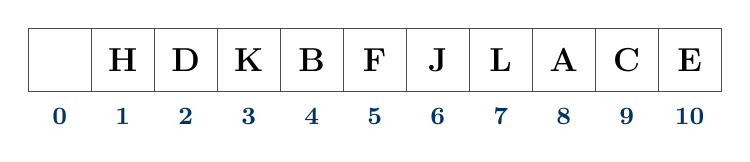
\begin{tikzpicture}
        % Định nghĩa style cho ô vuông
        \tikzstyle{cell} = [
            draw=black!70, 
            thin, 
            minimum width=0.8cm, 
            minimum height=0.8cm, 
            font=\bfseries\large, 
            anchor=west,
            outer sep=0pt
        ]
        
        % Ô đầu tiên (Index 0 - Rỗng)
        \node[cell] at (0,0) (c0) {};
        \node[below=0.1cm of c0, font=\small\bfseries, text=HUSTBlue] {0};
        
        % Các ô tiếp theo (Index 1-10)
        % Dữ liệu: H, D, K, B, F, J, L, A, C, E
        \foreach \val/\idx in {H/1, D/2, K/3, B/4, F/5, J/6, L/7, A/8, C/9, E/10} {
            \node[cell] at (\idx*0.8, 0) (c\idx) {\val};
            \node[below=0.1cm of c\idx, font=\small\bfseries, text=HUSTBlue] {\idx};
        }
    \end{tikzpicture}
    }

    \vspace{0.4cm}

    % --- 2. VẼ BẢNG ---
    % Tăng chiều cao dòng
    \renewcommand{\arraystretch}{1.4}
    \setlength{\tabcolsep}{12pt} 
    
    \resizebox{0.6\textwidth}{!}{%
    \begin{tabular}{|c|c|c|}
        \hline
        % Header bảng (In đậm thay vì tô màu nền để tránh lỗi)
        \textbf{Để tìm} & \textbf{Sử dụng} & \textbf{Hạn chế} \\ 
        \hline
        
        Con trái của A[i] & A[$2*i$] & $2*i \le n$ \\ 
        \hline
        
        Con phải của A[i] & A[$2*i + 1$] & $2*i + 1 \le n$ \\ 
        \hline
        
        Cha của A[i] & A[$i/2$] & $i > 1$ \\ 
        \hline
        
        Gốc & A[1] & A khác rỗng \\ 
        \hline
        
        Thử A[i] là lá? & True & $2*i > n$ \\ 
        \hline
    \end{tabular}
    }

\end{frame}

\begin{frame}[t]{3. CÂY NHỊ PHÂN}
    \begin{itemize}
        \item \textbf{3.1. Biểu diễn cây nhị phân}
        \begin{itemize}
            \item \textbf{Biểu diễn sử dụng con trỏ}
        \end{itemize}
    \end{itemize}
    \centering
    \large
    Mỗi nút của cây sẽ có con trỏ đến con trái và con trỏ đến con phải:
    \vspace{0.4cm}

    % --- 1. HÌNH VẼ MINH HỌA NÚT ---
    \resizebox{0.8\textwidth}{!}{%
    \begin{tikzpicture}
        % Style cho các ô vuông: Viền xanh, nền vàng
        \tikzstyle{box} = [
            draw=blue, 
            thick, 
            fill=yellow!60, 
            minimum width=1.5cm, 
            minimum height=1.2cm, 
            outer sep=0pt,
            font=\bfseries
        ]

        % Vẽ 3 ô liền nhau
        \node[box] (left) {};
        \node[box, right=0cm of left] (key) {key};
        \node[box, right=0cm of key] (right) {};

        % Mũi tên và nhãn
        % Mũi tên trái (đi ra từ tâm ô trái)
        \draw[blue, thick, -{Latex[length=3mm, width=2mm]}] (left.center) -- ++(-2.5, 0) 
            node[left] {\textbf{Trỏ đến con trái}};
            
        % Mũi tên phải (đi ra từ tâm ô phải)
        \draw[blue, thick, -{Latex[length=3mm, width=2mm]}] (right.center) -- ++(2.5, 0) 
            node[right] {\textbf{Trỏ đến con phải}};

        % Điểm nhấn (diamond) ở đầu mũi tên (như trong hình)
        \fill[blue] (left.center) circle (2pt); % Hoặc vẽ hình thoi nhỏ nếu muốn giống hệt
        \fill[blue] (right.center) circle (2pt);

    \end{tikzpicture}
    }

    \vspace{0.5cm}

    % --- 2. KHUNG CODE C++ ---
    % Sử dụng TikZ node để tạo khung viền xanh bao quanh code
    \resizebox{0.8\textwidth}{!}{%
    \begin{tikzpicture}
        \node[
            draw=HUSTBlue!70,   % Viền xanh nhạt hơn chút
            thick,
            align=left,         % Canh trái văn bản
            inner sep=10pt,     % Khoảng cách lề
            font=\large\ttfamily % Font monospaced
        ] {
            \textcolor{red}{struct} \textcolor{red}{Tnode} \{ \\
            \hspace{0.8cm} \textcolor{red}{DataType} \textcolor{red!80!black}{Item}; \textcolor{violet}{// DataType - kiểu dữ liệu của phần tử} \\
            \\
            \hspace{0.8cm} \textcolor{red}{struct} \textcolor{red}{Tnode} *\textcolor{red!80!black}{left}; \\
            \hspace{0.8cm} \textcolor{red}{struct} \textcolor{red}{Tnode} *\textcolor{red!80!black}{right}; \\
            \}; \\
            \textcolor{red}{typedef struct} \textcolor{red}{Tnode} \textcolor{red!80!black}{treeNode};
        };
    \end{tikzpicture}
    }

\end{frame}

\begin{frame}[fragile, t]{3. CÂY NHỊ PHÂN}
    \begin{itemize}
        \vspace{-0.2em}
        \item \textbf{3.1. Biểu diễn cây nhị phân}
        \begin{itemize}
            \item \textbf{Biểu diễn sử dụng con trỏ}
        \end{itemize}
    \end{itemize}
    
    \begin{columns}[T]
        % --- CỘT TRÁI: CÂY NHỊ PHÂN (HÌNH VẼ) ---
        \begin{column}{0.4\textwidth}
            \centering
            % Dùng scale thay vì resizebox để tránh lỗi
            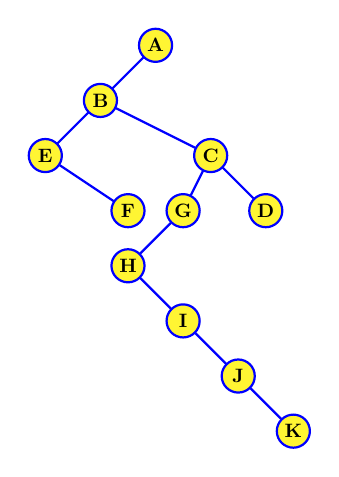
\begin{tikzpicture}[
                scale=0.7, transform shape,
                treenode/.style={
                    circle, 
                    draw=blue, 
                    fill=yellow!80, 
                    thick, 
                    font=\bfseries, 
                    minimum size=0.6cm,
                    inner sep=0pt
                },
                edge/.style={draw=blue, thick}
            ]
                \node[treenode] (A) at (1, 0) {A};
                \node[treenode] (B) at (0, -1) {B};
                \node[treenode] (C) at (2, -2) {C};
                \node[treenode] (E) at (-1, -2) {E};
                \node[treenode] (D) at (3, -3) {D};
                \node[treenode] (F) at (0.5, -3) {F}; 
                \node[treenode] (G) at (1.5, -3) {G}; 
                \node[treenode] (H) at (0.5, -4) {H}; 
                \node[treenode] (I) at (1.5, -5) {I}; 
                \node[treenode] (J) at (2.5, -6) {J}; 
                \node[treenode] (K) at (3.5, -7) {K}; 

                \draw[edge] (A) -- (B);
                \draw[edge] (B) -- (E);
                \draw[edge] (B) -- (C);
                \draw[edge] (C) -- (D);
                \draw[edge] (E) -- (F); 
                \draw[edge] (C) -- (G);
                \draw[edge] (G) -- (H);
                \draw[edge] (H) -- (I);
                \draw[edge] (I) -- (J);
                \draw[edge] (J) -- (K);
            \end{tikzpicture}
            \vspace{-0.1em}
            \par \textbf{Cây nhị phân}
        \end{column}
        
        % --- CỘT PHẢI: SƠ ĐỒ CON TRỎ ---
        \begin{column}{0.6\textwidth}
            \centering
            % Dùng scale thay vì resizebox
            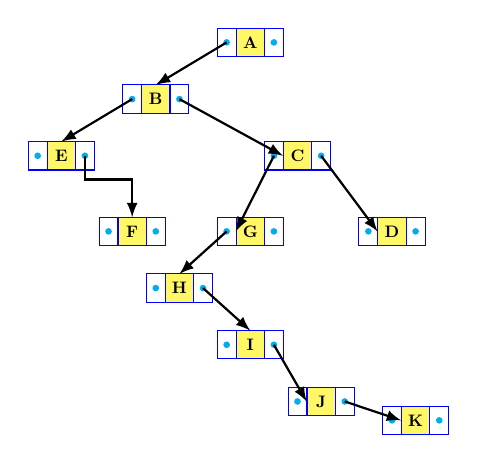
\begin{tikzpicture}[
                scale=0.6, transform shape,
                dsnode/.pic={
                    \node[draw=blue, fill=white, minimum width=0.4cm, minimum height=0.6cm] (-l) at (-0.5,0) {};
                    \fill[cyan] (-l.center) circle (2pt);
                    \node[draw=blue, fill=yellow!60, minimum width=0.6cm, minimum height=0.6cm, font=\bfseries] (-d) at (0,0) {#1};
                    \node[draw=blue, fill=white, minimum width=0.4cm, minimum height=0.6cm] (-r) at (0.5,0) {};
                    \fill[cyan] (-r.center) circle (2pt);
                    \coordinate (-top) at (0, 0.3);
                    \coordinate (-bottom) at (0, -0.3);
                },
                node distance=1.0cm,
                arrow/.style={->, >=latex, draw=black, thick}
            ]
                \path (2, 0) pic (A) {dsnode=A};
                \path (0, -1.2) pic (B) {dsnode=B};
                \path (-2, -2.4) pic (E) {dsnode=E};
                \path (3, -2.4) pic (C) {dsnode=C};
                \path (5, -4.0) pic (D) {dsnode=D};
                \path (-0.5, -4.0) pic (F) {dsnode=F};
                \path (2, -4.0) pic (G) {dsnode=G};
                \path (0.5, -5.2) pic (H) {dsnode=H};
                \path (2, -6.4) pic (I) {dsnode=I};
                \path (3.5, -7.6) pic (J) {dsnode=J};
                \path (5.5, -8.0) pic (K) {dsnode=K};

                \draw[arrow] (A-l.center) -- (B-top);
                \draw[arrow] (B-l.center) -- (E-top);
                \draw[arrow] (B-r.center) -- (C-d.west);
                \draw[arrow] (E-r.center) -- ++(0,-0.5) -| (F-top);
                \draw[arrow] (C-r.center) -- (D-d.west);
                \draw[arrow] (C-l.center) -- (G-d.west);
                \draw[arrow] (G-l.center) -- (H-top);
                \draw[arrow] (H-r.center) -- (I-top); 
                \draw[arrow] (I-r.center) -- (J-d.west);
                \draw[arrow] (J-r.center) -- (K-d.west);
            \end{tikzpicture}
            
            \par \textbf{Cây nhị phân biểu diễn bằng con trỏ}
        \end{column}
    \end{columns}
\end{frame}

\begin{frame}[fragile, t]{3. CÂY NHỊ PHÂN}
    \vspace{0.2cm}
    \begin{itemize}
        \item \textbf{3.2. Duyệt cây nhị phân}
        \begin{itemize}
            \item \textbf{Duyệt theo thứ tự trước}
        \end{itemize}
    \end{itemize}

    \vspace{0.3cm}
    
    \begin{columns}[T]
        % --- CỘT TRÁI ---
        \begin{column}{0.4\textwidth}
            \setlength{\fboxrule}{0.8pt}
            \fcolorbox{HUSTBlue}{white}{%
                % [t][5.5cm]: Căn trên (top) và chiều cao cố định 5.5cm
                \begin{minipage}[t][3.65cm]{0.9\textwidth}
                    \vspace{0.5cm} % Khoảng trống đệm phía trên
                    \begin{itemize}
                        \setlength{\itemsep}{0.8cm}
                        \item Thăm nút
                        \item Duyệt cây con trái
                        \item Duyệt cây con phải
                    \end{itemize}
                \end{minipage}
            }
        \end{column}
        
        % --- CỘT PHẢI ---
        \begin{column}{0.58\textwidth}
            % Sử dụng hộp chứa (lrbox) để tránh lỗi với minted
            \newsavebox{\codebox}
            \begin{lrbox}{\codebox}
                % Đặt chiều cao cố định 5.5cm giống bên trái
                \begin{minipage}[t][3.65cm]{0.95\textwidth}
                    \vspace{0.1cm}
                    \begin{minted}[fontsize=\small, breaklines]{c}
void printPreorder(treeNode *tree) {
   if( tree != NULL ) {
      printf("%s\n", tree->word);
      printPreorder(tree->left);
      printPreorder(tree->right);
   }
}
                    \end{minted}
                \end{minipage}
            \end{lrbox}

            \setlength{\fboxrule}{0.8pt}
            \fcolorbox{HUSTBlue}{white}{\usebox{\codebox}}
        \end{column}
    \end{columns}
\end{frame}

\begin{frame}[t]{3. CÂY NHỊ PHÂN}
    \vspace{0.2cm}
    \begin{itemize}
        \item \textbf{3.2. Duyệt cây nhị phân}
        \begin{itemize}
            \item \textbf{Duyệt theo thứ tự trước}
        \end{itemize}
    \end{itemize}

    \vspace{0.1cm}
    \centering
    
    \resizebox{0.6\textwidth}{!}{%
    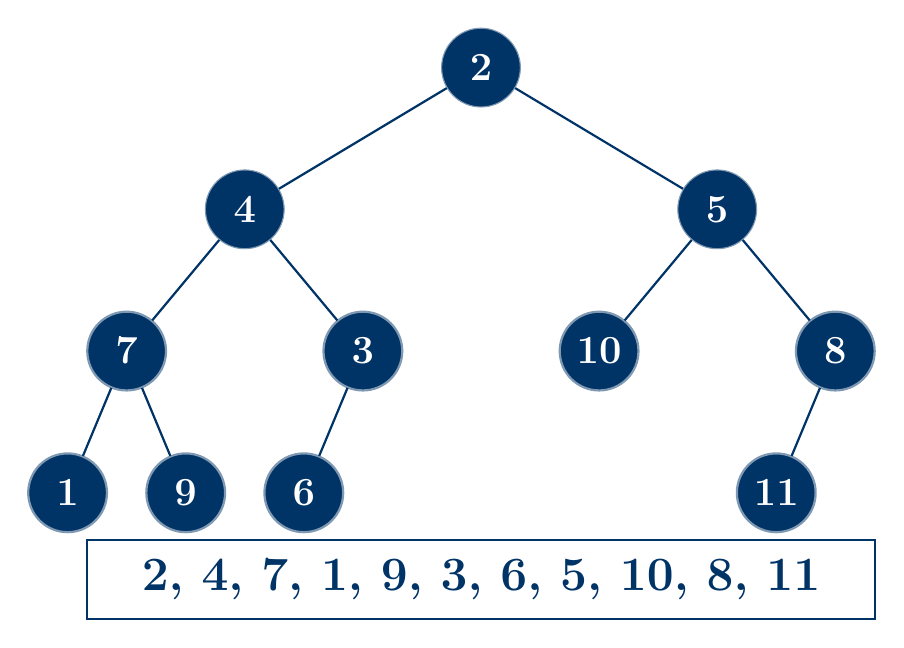
\begin{tikzpicture}[
        % Cấu hình khoảng cách các cấp
        level 1/.style={sibling distance=6cm, level distance=1.8cm},
        level 2/.style={sibling distance=3cm, level distance=1.8cm},
        level 3/.style={sibling distance=1.5cm, level distance=1.8cm},
        % Style cho nút: Tròn, nền xanh đậm, chữ trắng
        treenode/.style={
            circle, 
            draw=HUSTBlue!50, 
            % ĐỔI MÀU NỀN: Sang màu xanh đậm HUSTBlue
            fill=HUSTBlue, 
            text=white, 
            font=\bfseries\Large, 
            minimum size=1.0cm,
            inner sep=0pt
        },
        edge from parent/.style={draw=HUSTBlue, thick}
    ]
        % --- VẼ CÂY ---
        % Root: 2
        \node[treenode] {2}
            % Nhánh trái: 4
            child { node[treenode] {4}
                % Con của 4: 7, 3
                child { node[treenode] {7}
                    child { node[treenode] {1} }
                    child { node[treenode] {9} }
                }
                child { node[treenode] {3}
                    child { node[treenode] {6} }
                    child[missing] % Để tạo khoảng trống bên phải nút 3
                }
            }
            % Nhánh phải: 5
            child { node[treenode] {5}
                % Con của 5: 10, 8
                child { node[treenode] {10} }
                child { node[treenode] {8}
                    child { node[treenode] {11} }
                    child[missing] % Để tạo khoảng trống bên phải nút 8
                }
            };

        % --- VẼ HỘP KẾT QUẢ ---
        % Vẽ thủ công ở vị trí y = -6.5 (dưới đáy cây)
        \node[
            draw=HUSTBlue, 
            thick,
            fill=white,
            minimum width=10cm, 
            minimum height=1cm, 
            font=\bfseries\LARGE\color{HUSTBlue}
        ] at (0, -6.5) {2, 4, 7, 1, 9, 3, 6, 5, 10, 8, 11};

    \end{tikzpicture}
    }
\end{frame}

\begin{frame}[fragile, t]{3. CÂY NHỊ PHÂN}
    \vspace{0.2cm}
    \begin{itemize}
        \item \textbf{3.2. Duyệt cây nhị phân}
        \begin{itemize}
            \item \textbf{Duyệt theo thứ tự giữa}
        \end{itemize}
    \end{itemize}

    \vspace{0.3cm}
    
    \begin{columns}[T]
        % --- CỘT TRÁI: GIẢI THUẬT ---
        \begin{column}{0.4\textwidth}
            \setlength{\fboxrule}{0.8pt}
            \fcolorbox{HUSTBlue}{white}{%
                % Giữ nguyên chiều cao 4.2cm để đồng bộ với slide trước
                \begin{minipage}[t][4.2cm]{0.9\textwidth}
                    \vspace{0.3cm}
                    \begin{itemize}
                        \setlength{\itemsep}{0.6cm} 
                        
                        % Thứ tự Inorder: Trái -> Gốc -> Phải
                        \item Duyệt cây con trái
                        
                        \item Thăm nút
                        
                        \item Duyệt cây con phải
                        
                    \end{itemize}
                \end{minipage}
            }
        \end{column}
        
        % --- CỘT PHẢI: CODE C ---
        \begin{column}{0.58\textwidth}
            % Sử dụng kỹ thuật lrbox để tránh lỗi minted trong fcolorbox
            \newsavebox{\codeboxInorder}
            \begin{lrbox}{\codeboxInorder}
                \begin{minipage}[t][4.2cm]{0.95\textwidth}
                    \vspace{0.1cm}
                    \begin{minted}[fontsize=\small, breaklines]{c}
void printInorder(treeNode *tree) {
   if( tree != NULL ) {
      printInorder(tree->left);
      printf("%s\n", tree->word);
      printInorder(tree->right);
   }
}
                    \end{minted}
                \end{minipage}
            \end{lrbox}

            \setlength{\fboxrule}{0.8pt}
            \fcolorbox{HUSTBlue}{white}{\usebox{\codeboxInorder}}
        \end{column}
    \end{columns}
\end{frame}

\begin{frame}[t]{3. CÂY NHỊ PHÂN}
    \vspace{0.2cm}
    \begin{itemize}
        \item \textbf{3.2. Duyệt cây nhị phân}
        \begin{itemize}
            \item \textbf{Duyệt theo thứ tự giữa}
        \end{itemize}
    \end{itemize}

    \vspace{0.1cm}
    \centering
    
    % Giữ nguyên kích thước 0.7 để đồng bộ với các slide trước
    \resizebox{0.6\textwidth}{!}{%
    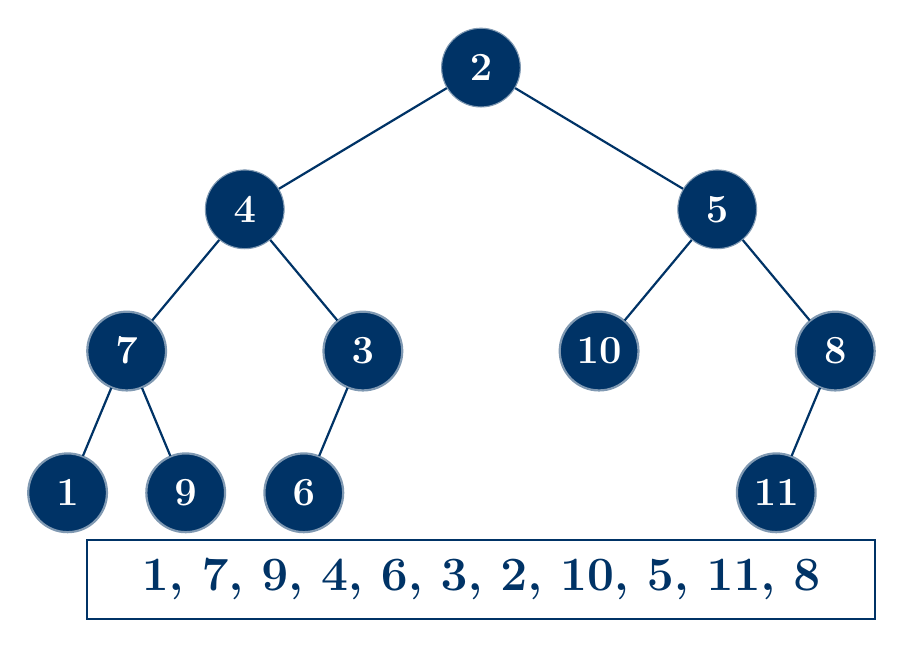
\begin{tikzpicture}[
        % Cấu hình khoảng cách các cấp
        level 1/.style={sibling distance=6cm, level distance=1.8cm},
        level 2/.style={sibling distance=3cm, level distance=1.8cm},
        level 3/.style={sibling distance=1.5cm, level distance=1.8cm},
        % Style cho nút: Tròn, nền xanh đậm HUSTBlue, chữ trắng
        treenode/.style={
            circle, 
            draw=HUSTBlue!50, 
            fill=HUSTBlue, 
            text=white, 
            font=\bfseries\Large, 
            minimum size=1.0cm,
            inner sep=0pt
        },
        edge from parent/.style={draw=HUSTBlue, thick}
    ]
        % --- VẼ CÂY (Cấu trúc giống slide 49) ---
        % Root: 2
        \node[treenode] {2}
            % Nhánh trái: 4
            child { node[treenode] {4}
                % Con của 4: 7, 3
                child { node[treenode] {7}
                    child { node[treenode] {1} }
                    child { node[treenode] {9} }
                }
                child { node[treenode] {3}
                    child { node[treenode] {6} }
                    child[missing] % Để 6 nằm bên trái
                }
            }
            % Nhánh phải: 5
            child { node[treenode] {5}
                % Con của 5: 10, 8
                child { node[treenode] {10} }
                child { node[treenode] {8}
                    child { node[treenode] {11} }
                    child[missing] % Để 11 nằm bên trái
                }
            };

        % --- VẼ HỘP KẾT QUẢ ---
        % Kết quả duyệt Inorder: Trái -> Gốc -> Phải
        \node[
            draw=HUSTBlue, 
            thick,
            fill=white,
            minimum width=10cm, 
            minimum height=1cm, 
            font=\bfseries\LARGE\color{HUSTBlue}
        ] at (0, -6.5) {1, 7, 9, 4, 6, 3, 2, 10, 5, 11, 8};

    \end{tikzpicture}
    }
\end{frame}

\begin{frame}[fragile, t]{3. CÂY NHỊ PHÂN}
    \vspace{0.2cm}
    \begin{itemize}
        \item \textbf{3.2. Duyệt cây nhị phân}
        \begin{itemize}
            \item \textbf{3.2.3. Duyệt theo thứ tự sau}
        \end{itemize}
    \end{itemize}

    \vspace{0.3cm}
    
    \begin{columns}[T]
        % --- CỘT TRÁI: GIẢI THUẬT (Đã chỉnh lại cho đúng logic Postorder) ---
        \begin{column}{0.4\textwidth}
            \setlength{\fboxrule}{0.8pt}
            \fcolorbox{HUSTBlue}{white}{%
                % Giữ nguyên chiều cao 4.2cm để đồng bộ với các slide trước
                \begin{minipage}[t][4.2cm]{0.9\textwidth}
                    \vspace{0.3cm}
                    \begin{itemize}
                        \setlength{\itemsep}{0.6cm} 
                        
                        % Thứ tự Postorder: Trái -> Phải -> Gốc
                        \item Duyệt cây con trái
                        
                        \item Duyệt cây con phải
                        
                        \item Thăm nút
                        
                    \end{itemize}
                \end{minipage}
            }
        \end{column}
        
        % --- CỘT PHẢI: CODE C ---
        \begin{column}{0.58\textwidth}
            % Sử dụng kỹ thuật lrbox để tránh lỗi minted trong fcolorbox
            \newsavebox{\codeboxPostorder}
            \begin{lrbox}{\codeboxPostorder}
                \begin{minipage}[t][4.2cm]{0.95\textwidth}
                    \vspace{0.1cm}
                    \begin{minted}[fontsize=\small, breaklines]{c}
void printPostorder(treeNode *tree) {
   if( tree != NULL ) {
      printPostorder(tree->left);
      printPostorder(tree->right);
      printf("%s\n", tree->word);
   }
}
                    \end{minted}
                \end{minipage}
            \end{lrbox}

            \setlength{\fboxrule}{0.8pt}
            \fcolorbox{HUSTBlue}{white}{\usebox{\codeboxPostorder}}
        \end{column}
    \end{columns}
\end{frame}

\begin{frame}[t]{3. CÂY NHỊ PHÂN}
    \vspace{0.2cm}
    \begin{itemize}
        \item \textbf{3.2. Duyệt cây nhị phân}
        \begin{itemize}
            \item \textbf{Duyệt theo thứ tự sau}
        \end{itemize}
    \end{itemize}

    \vspace{0.1cm}
    \centering
    
    % Giữ nguyên kích thước để đồng bộ
    \resizebox{0.6\textwidth}{!}{%
    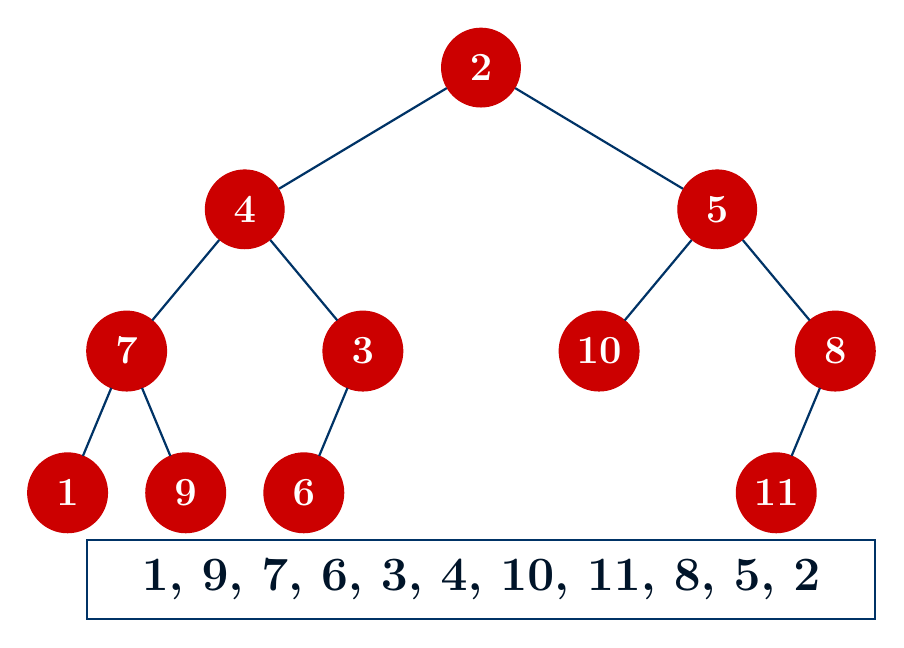
\begin{tikzpicture}[
        % Cấu hình khoảng cách
        level 1/.style={sibling distance=6cm, level distance=1.8cm},
        level 2/.style={sibling distance=3cm, level distance=1.8cm},
        level 3/.style={sibling distance=1.5cm, level distance=1.8cm},
        % Style cho nút: Tròn, nền ĐỎ đậm, chữ trắng
        treenode/.style={
            circle, 
            draw=red!80!black, 
            fill=red!80!black, % Màu đỏ như trong hình
            text=white, 
            font=\bfseries\Large, 
            minimum size=1.0cm,
            inner sep=0pt
        },
        edge from parent/.style={draw=HUSTBlue, thick}
    ]
        % --- VẼ CÂY ---
        % Root: 2
        \node[treenode] {2}
            % Nhánh trái: 4
            child { node[treenode] {4}
                % Con của 4: 7, 3
                child { node[treenode] {7}
                    child { node[treenode] {1} }
                    child { node[treenode] {9} }
                }
                child { node[treenode] {3}
                    child { node[treenode] {6} }
                    child[missing] % Khoảng trống để 6 nằm bên trái
                }
            }
            % Nhánh phải: 5
            child { node[treenode] {5}
                % Con của 5: 10, 8
                child { node[treenode] {10} }
                child { node[treenode] {8}
                    child { node[treenode] {11} }
                    child[missing] % Khoảng trống để 11 nằm bên trái
                }
            };

        % --- VẼ HỘP KẾT QUẢ ---
        % Kết quả duyệt Postorder: 1, 9, 7, 6, 3, 4, 10, 11, 8, 5, 2
        \node[
            draw=HUSTBlue, 
            thick,
            fill=white,
            minimum width=10cm, 
            minimum height=1cm, 
            font=\bfseries\LARGE\color{HUSTBlue!40!black}
        ] at (0, -6.5) {1, 9, 7, 6, 3, 4, 10, 11, 8, 5, 2};

    \end{tikzpicture}
    }
\end{frame}
\section{Định nghĩa chiều cao và độ sâu của nút}
\begin{frame}[t]{1. ĐỊNH NGHĨA CHIỀU CAO VÀ ĐỘ SÂU CỦA NÚT}
    \vspace{0.2cm}
    \begin{itemize}
        \item \textbf{1.1. Định nghĩa}
        \vspace{0.3cm}
        
        \item \textbf{Chiều cao} (\textit{height}) của nút trên cây là bằng độ dài của đường đi dài nhất từ nút đó đến lá cộng 1.
        \vspace{0.2cm}
        
        \begin{itemize}
            \item Chiều cao của cây (\textit{height of a tree}) là chiều cao của gốc.
        \end{itemize}
        \vspace{0.3cm}
        
        \item \textbf{Độ sâu/mức} (\textit{depth/level}) của nút là bằng 1 cộng với độ dài của đường đi duy nhất từ gốc đến nó.
    \end{itemize}
\end{frame}

\begin{frame}{1. ĐỊNH NGHĨA CHIỀU CAO VÀ ĐỘ SÂU CỦA NÚT}
    \textbf{1.2. Ví dụ}
    \vspace{0.2cm}

    \centering
    % Dùng resizebox để ép hình vừa khít 85% chiều rộng trang
    % Dấu % ở cuối các dòng là để tránh sinh ra khoảng trắng thừa
    \resizebox{0.85\textwidth}{!}{%
    \begin{tikzpicture}[
        treenode/.style={circle, draw=myblue, very thick, fill=yellow!50, font=\bfseries\color{myblue}\large, minimum size=1cm, inner sep=2pt},
        edge/.style={draw=myblue, thick}
    ]
    % --- Vẽ cây ---
    \node[treenode] (A) at (0, 0) {A};
    \node[treenode] (B) at (-3, -2) {B};
    \node[treenode] (C) at (3, -2) {C};
    \draw[edge] (A) -- (B);
    \draw[edge] (A) -- (C);
    \node[treenode] (D) at (-4, -4) {D};
    \node[treenode] (E) at (-2, -4) {E};
    \node[treenode] (F) at (2, -4) {F};
    \node[treenode] (G) at (4, -4) {G};
    \draw[edge] (B) -- (D);
    \draw[edge] (B) -- (E);
    \draw[edge] (C) -- (F);
    \draw[edge] (C) -- (G);
    \node[treenode] (H) at (-4.7, -6) {H};
    \node[treenode] (I) at (-3.3, -6) {I};
    \draw[edge] (D) -- (H);
    \draw[edge] (D) -- (I);
    % --- Chú thích bên phải (Mức/Độ sâu) ---
    \begin{scope}[every node/.style={anchor=west, font=\large}]
        \node at (5.5, 0) {Mức 1 (Độ sâu 1)};
        \node at (5.5, -2) {Mức 2 (Độ sâu 2)};
        \node at (5.5, -4) {Mức 3 (Độ sâu 3)};
        \node at (5.5, -6) {Mức 4 (Độ sâu 4)};
    \end{scope}
    % --- Chú thích bên trái (Chiều cao) ---
    \draw[decorate, decoration={brace, amplitude=12pt, mirror}, very thick, myblue] (-6, 0.5) -- (-6, -6.5) node[midway, left=15pt, align=center, font=\bfseries\large\color{myblue}] {Chiều cao\\của cây = 4};
    \end{tikzpicture}%
    }
\end{frame}

\begin{frame}{1. ĐỊNH NGHĨA CHIỀU CAO VÀ ĐỘ SÂU CỦA NÚT}
    \textbf{1.2. Ví dụ}
    \vspace{0.2cm}

    \centering
    % Resize để hình vừa khít slide
    \resizebox{0.8\textwidth}{!}{%
    \begin{tikzpicture}[
        % Style cho các node
        treenode/.style={
            circle, 
            draw=blue!40!black, 
            fill=blue!60!white, % Màu xanh dương nhạt hơn chút cho giống hình
            text=white, 
            font=\bfseries\large, 
            minimum size=1cm,
            inner sep=0pt
        },
        % Style cho cạnh nối
        edge/.style={
            draw=blue!40!black, 
            thick
        },
        % Style cho label bên trái (màu đỏ)
        label-red/.style={
            text=red!80!black, 
            font=\bfseries\large, 
            anchor=west
        },
        % Style cho label bên phải (màu đen/xanh)
        label-blue/.style={
            text=black, 
            font=\large, 
            anchor=west
        }
    ]

        % --- 1. VẼ CÂY ---
        % Tọa độ được căn chỉnh thủ công để khớp với cấu trúc trong hình
        
        % Level 1 (Root)
        \node[treenode] (n7) at (0, 0) {7};

        % Level 2
        \node[treenode] (n3) at (-3, -2) {3};
        \node[treenode] (n10) at (0, -2) {10};
        \node[treenode] (n4) at (4, -2) {4};

        % Level 3
        \node[treenode] (n8) at (-3.8, -4) {8};
        \node[treenode] (n12) at (-1.8, -4) {12};
        \node[treenode] (n11) at (2.5, -4) {11};
        \node[treenode] (n2) at (5.5, -4) {2};

        % Level 4
        \node[treenode] (n6) at (-4.5, -6) {6};
        \node[treenode] (n5) at (-2.8, -6) {5};
        \node[treenode] (n1) at (-0.3, -6) {1};

        % Level 5
        \node[treenode] (n9) at (-3.8, -8) {9};

        % --- 2. VẼ CẠNH ---
        \draw[edge] (n7) -- (n3);
        \draw[edge] (n7) -- (n10);
        \draw[edge] (n7) -- (n4);

        \draw[edge] (n3) -- (n8);
        \draw[edge] (n3) -- (n12);

        \draw[edge] (n4) -- (n11);
        \draw[edge] (n4) -- (n2);

        \draw[edge] (n8) -- (n6);
        \draw[edge] (n8) -- (n5);
        \draw[edge] (n12) -- (n1);

        \draw[edge] (n5) -- (n9);

        % --- 3. CHÚ THÍCH ĐỘ CAO (BÊN TRÁI - MŨI TÊN ĐỎ) ---
        % Vẽ mũi tên đỏ đi lên
        \draw[->, >=latex, line width=2pt, red!80!black] (-7, -8) -- (-7, 0.5);

        % Các nhãn độ cao
        \node[label-red] at (-6.8, 0) {độ cao $h = 5$};
        \node[label-red] at (-6.8, -2) {độ cao $= 4$};
        \node[label-red] at (-6.8, -4) {độ cao $= 3$};
        \node[label-red] at (-6.8, -6) {$h = 2$};
        
        % Nhãn h=1 có nền xanh
        \node[fill=blue!80!black, text=yellow, font=\bfseries\large, anchor=west] at (-7.5, -8) {độ cao $h=1$};


        % --- 4. CHÚ THÍCH ĐỘ SÂU (BÊN PHẢI - MŨI TÊN XANH) ---
        % Vẽ mũi tên xanh đi xuống
        \draw[->, >=latex, line width=2pt, blue] (6.5, 0) -- (6.5, -8);

        % Nhãn độ sâu 1 có nền xanh
        \node[fill=blue, text=yellow, font=\bfseries\large, anchor=west] at (6.5, 0) {độ sâu 1};
        
        % Các nhãn độ sâu khác
        \node[label-blue] at (6.8, -2) {độ sâu 2};
        \node[label-blue] at (6.8, -4) {độ sâu 3};
        \node[label-blue] at (6.8, -6) {độ sâu 4};
        \node[label-blue] at (6.8, -8) {độ sâu 5};

        % --- 5. LABEL CUỐI CÙNG ---
        \node[font=\large] at (0, -8) {Độ cao của cây là 5};

    \end{tikzpicture}%
    }
\end{frame}
\section{Thuật toán tìm chiều cao và độ sâu}
\begin{frame}[fragile]{2. THUẬT TOÁN TÌM CHIỀU CAO VÀ ĐỘ SÂU}
    \begin{itemize}
        \item Cấu trúc dữ liệu biểu diễn cây
    \end{itemize}

    \centering
    % 1. Tạo hộp chứa code (để tránh lỗi xung đột giữa minted và fcolorbox)
    \newsavebox{\codeboxStruct}
    \begin{lrbox}{\codeboxStruct}
        \begin{minipage}{0.6\textwidth}
            \vspace{0.2cm}
            % Code C++ định nghĩa struct
            \begin{minted}[fontsize=\large, breaklines]{cpp}
struct Node{
    int id;
    Node* leftMostChild;
    Node* rightSibling;
};
Node* root;
            \end{minted}

        \end{minipage}
    \end{lrbox}

    % 2. Vẽ khung viền bao quanh hộp code
    \setlength{\fboxrule}{1pt} % Độ dày viền
    \fcolorbox{HUSTBlue}{white}{%
        \usebox{\codeboxStruct}
    }
\end{frame}

\begin{frame}[fragile]{2. THUẬT TOÁN TÌM CHIỀU CAO VÀ ĐỘ SÂU}
    \textbf{2.1. Tìm độ cao của một nút}
    \begin{itemize}
        \item Độ cao của một nút
    \end{itemize}

    \begin{columns}[T]
        % --- CỘT TRÁI: HÌNH MINH HỌA ---
        \begin{column}{0.5\textwidth}
            \centering
            \resizebox{0.8\textwidth}{!}{%
            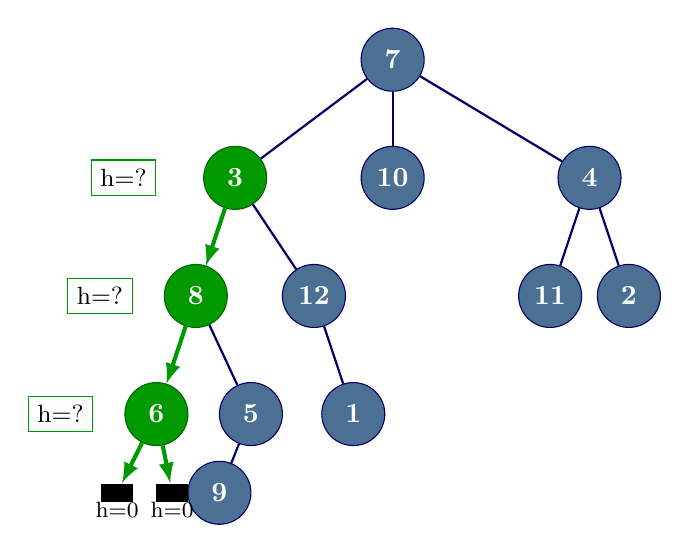
\begin{tikzpicture}[
                % Style cho các loại node
                stdnode/.style={circle, draw=blue!40!black, fill=HUSTBlue!70, text=white, font=\bfseries, minimum size=0.8cm, inner sep=0pt},
                highlightnode/.style={circle, draw=green!40!black, fill=green!60!black, text=white, font=\bfseries, minimum size=0.8cm, inner sep=0pt},
                nullnode/.style={rectangle, fill=black, minimum width=0.4cm, minimum height=0.2cm},
                % Style cạnh
                edge/.style={draw=blue!40!black, thick},
                arrowedge/.style={->, >=latex, draw=green!60!black, line width=1.5pt},
                % Style nhãn h=?
                hlabel/.style={draw=green!60!black, text=black, fill=white, font=\small, anchor=east}
            ]
                % --- VẼ CÂY ---
                % Root
                \node[stdnode] (n7) at (0, 0) {7};

                % Level 2
                \node[highlightnode] (n3) at (-2, -1.5) {3};
                \node[stdnode] (n10) at (0, -1.5) {10};
                \node[stdnode] (n4) at (2.5, -1.5) {4};

                % Level 3
                \node[highlightnode] (n8) at (-2.5, -3) {8};
                \node[stdnode] (n12) at (-1, -3) {12};
                \node[stdnode] (n11) at (2, -3) {11};
                \node[stdnode] (n2) at (3, -3) {2};

                % Level 4
                \node[highlightnode] (n6) at (-3, -4.5) {6};
                \node[stdnode] (n5) at (-1.8, -4.5) {5};
                \node[stdnode] (n1) at (-0.5, -4.5) {1};

                % Level 5 (Node 9)
                \node[stdnode] (n9) at (-2.2, -5.5) {9};
                
                % Base case (Null nodes dưới node 6)
                \node[nullnode] (null1) at (-3.5, -5.5) {};
                \node[nullnode] (null2) at (-2.8, -5.5) {};


                % --- VẼ CẠNH ---
                % Cạnh thường
                \draw[edge] (n7) -- (n3); \draw[edge] (n7) -- (n10); \draw[edge] (n7) -- (n4);
                \draw[edge] (n3) -- (n12);
                \draw[edge] (n8) -- (n5);
                \draw[edge] (n12) -- (n1);
                \draw[edge] (n4) -- (n11); \draw[edge] (n4) -- (n2);
                \draw[edge] (n5) -- (n9);

                % Cạnh đệ quy (Mũi tên xanh)
                \draw[arrowedge] (n3) -- (n8);
                \draw[arrowedge] (n8) -- (n6);
                \draw[arrowedge] (n6) -- (null1);
                \draw[arrowedge] (n6) -- (null2);

                % --- NHÃN (LABELS) ---
                \node[hlabel] at (-3, -1.5) {h=?};
                \node[hlabel] at (-3.3, -3) {h=?};
                \node[hlabel] at (-3.8, -4.5) {h=?};
                
                \node[font=\footnotesize, below] at (null1) {h=0};
                \node[font=\footnotesize, below] at (null2) {h=0};

            \end{tikzpicture}
            }
        \end{column}
        
        % --- CỘT PHẢI: CODE ---
        \begin{column}{0.5\textwidth}
            \newsavebox{\codeboxHeight}
            \begin{lrbox}{\codeboxHeight}
                \begin{minipage}{0.95\textwidth}
                    \vspace{0.1cm}
                    \begin{minted}[fontsize=\scriptsize, breaklines]{cpp}
int height(Node* p){
   if(p == NULL) return 0;
   int maxh = 0;
   Node* q = p->leftMostChild;
   while(q != NULL){
      int h = height(q);
      if(h > maxh) maxh = h;
      q = q->rightSibling;
   }
   return maxh + 1;
}
                    \end{minted}
                \end{minipage}
            \end{lrbox}

            \setlength{\fboxrule}{0.8pt}
            \fcolorbox{HUSTBlue}{white}{\usebox{\codeboxHeight}}
        \end{column}
    \end{columns}
\end{frame}

	\begin{frame}[fragile]{2. THUẬT TOÁN TÌM CHIỀU CAO VÀ ĐỘ SÂU}
    \textbf{2.1. Tìm độ cao của một nút}
    \begin{itemize}
        \item Độ cao của một nút
    \end{itemize}

    \begin{columns}[T]
        % --- CỘT TRÁI: HÌNH MINH HỌA ---
        \begin{column}{0.5\textwidth}
            \centering
            \resizebox{1.0\textwidth}{!}{%
            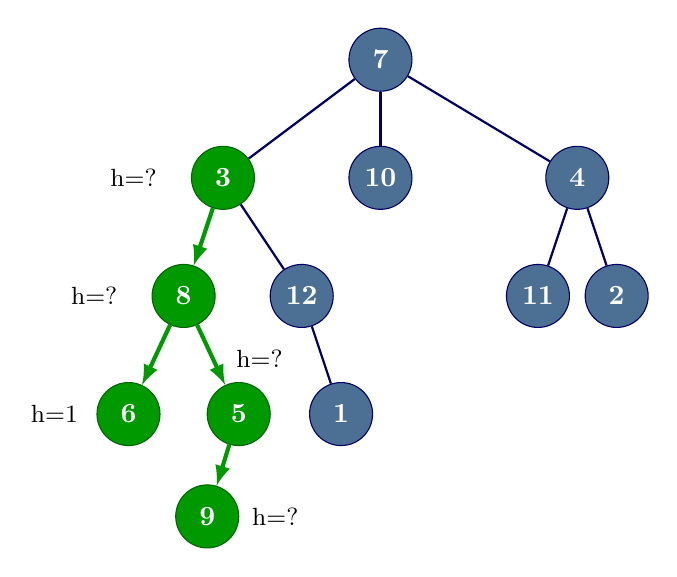
\begin{tikzpicture}[
                % Style cho các loại node
                stdnode/.style={circle, draw=blue!40!black, fill=HUSTBlue!70, text=white, font=\bfseries, minimum size=0.8cm, inner sep=0pt},
                highlightnode/.style={circle, draw=green!40!black, fill=green!60!black, text=white, font=\bfseries, minimum size=0.8cm, inner sep=0pt},
                % Style cạnh
                edge/.style={draw=blue!40!black, thick},
                arrowedge/.style={->, >=latex, draw=green!60!black, line width=1.5pt},
                % Style nhãn h=?
                hlabel/.style={draw=white, text=black, fill=white, font=\small, anchor=east, inner sep=1pt}
            ]
                % --- VẼ CÂY ---
                % Root
                \node[stdnode] (n7) at (0, 0) {7};

                % Level 2
                \node[highlightnode] (n3) at (-2, -1.5) {3};
                \node[stdnode] (n10) at (0, -1.5) {10};
                \node[stdnode] (n4) at (2.5, -1.5) {4};

                % Level 3
                \node[highlightnode] (n8) at (-2.5, -3) {8};
                \node[stdnode] (n12) at (-1, -3) {12};
                \node[stdnode] (n11) at (2, -3) {11};
                \node[stdnode] (n2) at (3, -3) {2};

                % Level 4
                \node[highlightnode] (n6) at (-3.2, -4.5) {6}; % Node 6 (Leaf)
                \node[highlightnode] (n5) at (-1.8, -4.5) {5}; % Node 5 (Next sibling)
                \node[stdnode] (n1) at (-0.5, -4.5) {1};

                % Level 5 (Node 9)
                \node[highlightnode] (n9) at (-2.2, -5.8) {9}; % Node 9 (Child of 5)

                % --- VẼ CẠNH ---
                % Cạnh thường
                \draw[edge] (n7) -- (n3); \draw[edge] (n7) -- (n10); \draw[edge] (n7) -- (n4);
                \draw[edge] (n3) -- (n12);
                \draw[edge] (n12) -- (n1);
                \draw[edge] (n4) -- (n11); \draw[edge] (n4) -- (n2);

                % Cạnh đệ quy (Mũi tên xanh) - Đường đi của thuật toán
                \draw[arrowedge] (n3) -- (n8);
                \draw[arrowedge] (n8) -- (n6); % Xuống con đầu tiên
                \draw[arrowedge] (n8) -- (n5); % Sang anh em kế tiếp
                \draw[arrowedge] (n5) -- (n9); % Xuống con của 5

                % --- NHÃN (LABELS) ---
                \node[hlabel] at (-2.8, -1.5) {h=?};
                \node[hlabel] at (-3.3, -3) {h=?};
                
                % Node 6 là lá, đã tính được h=1
                \node[hlabel, anchor=east] at (-3.8, -4.5) {h=1};
                
                % Node 5 đang xét
                \node[hlabel, anchor=east] at (-1.2, -3.8) {h=?};
                
                % Node 9 đang xét
                \node[hlabel, anchor=east] at (-1, -5.8) {h=?};

            \end{tikzpicture}
            }
        \end{column}
        
        % --- CỘT PHẢI: CODE ---
        \begin{column}{0.5\textwidth}
            \newsavebox{\codeboxHeightTwo}
            \begin{lrbox}{\codeboxHeightTwo}
                \begin{minipage}{0.95\textwidth}
                    \vspace{0.1cm}
                    \begin{minted}[fontsize=\scriptsize, breaklines]{cpp}
int height(Node* p){
   if(p == NULL) return 0;
   int maxh = 0;
   Node* q = p->leftMostChild;
   while(q != NULL){
      int h = height(q);
      if(h > maxh) maxh = h;
      q = q->rightSibling;
   }
   return maxh + 1;
}
                    \end{minted}
                \end{minipage}
            \end{lrbox}

            \setlength{\fboxrule}{0.8pt}
            \fcolorbox{HUSTBlue}{white}{\usebox{\codeboxHeightTwo}}
        \end{column}
    \end{columns}
\end{frame}

\begin{frame}[fragile]{2. THUẬT TOÁN TÌM CHIỀU CAO VÀ ĐỘ SÂU}
    \textbf{2.1. Tìm độ cao của một nút}
    \begin{itemize}
        \item Độ cao của một nút
    \end{itemize}

    \begin{columns}[T]
        % --- CỘT TRÁI: HÌNH MINH HỌA ---
        \begin{column}{0.5\textwidth}
            \centering
            \resizebox{1.0\textwidth}{!}{%
            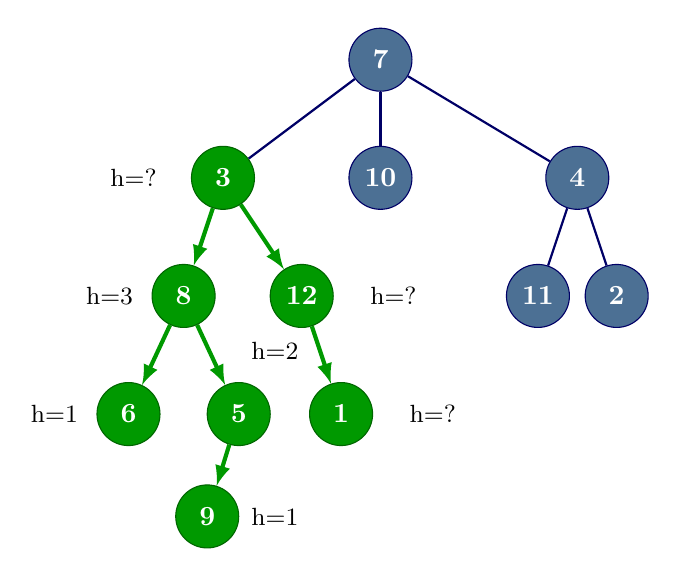
\begin{tikzpicture}[
                % Style giống hệt mẫu bạn cung cấp
                stdnode/.style={circle, draw=blue!40!black, fill=HUSTBlue!70, text=white, font=\bfseries, minimum size=0.8cm, inner sep=0pt},
                highlightnode/.style={circle, draw=green!40!black, fill=green!60!black, text=white, font=\bfseries, minimum size=0.8cm, inner sep=0pt},
                % Style cạnh
                edge/.style={draw=blue!40!black, thick},
                arrowedge/.style={->, >=latex, draw=green!60!black, line width=1.5pt},
                % Style nhãn
                hlabel/.style={draw=white, text=black, fill=white, font=\small, anchor=east, inner sep=1pt}
            ]
                % --- VẼ CÂY ---
                % Root
                \node[stdnode] (n7) at (0, 0) {7};

                % Level 2
                \node[highlightnode] (n3) at (-2, -1.5) {3};
                \node[stdnode] (n10) at (0, -1.5) {10};
                \node[stdnode] (n4) at (2.5, -1.5) {4};

                % Level 3
                \node[highlightnode] (n8) at (-2.5, -3) {8};   % Đã xong
                \node[highlightnode] (n12) at (-1, -3) {12};  % Đang xét
                \node[stdnode] (n11) at (2, -3) {11};
                \node[stdnode] (n2) at (3, -3) {2};

                % Level 4
                \node[highlightnode] (n6) at (-3.2, -4.5) {6}; % Đã xong
                \node[highlightnode] (n5) at (-1.8, -4.5) {5}; % Đã xong
                \node[highlightnode] (n1) at (-0.5, -4.5) {1}; % Đang xét

                % Level 5
                \node[highlightnode] (n9) at (-2.2, -5.8) {9}; % Đã xong

                % --- VẼ CẠNH ---
                % Cạnh thường (chưa duyệt)
                \draw[edge] (n7) -- (n3); \draw[edge] (n7) -- (n10); \draw[edge] (n7) -- (n4);
                \draw[edge] (n4) -- (n11); \draw[edge] (n4) -- (n2);

                % Cạnh đệ quy (Mũi tên xanh)
                % Nhánh con của 3: Đã xong nhánh 8
                \draw[arrowedge] (n3) -- (n8);
                \draw[arrowedge] (n8) -- (n6);
                \draw[arrowedge] (n8) -- (n5);
                \draw[arrowedge] (n5) -- (n9);
                
                % Nhánh con của 3: Đang xét nhánh 12
                \draw[arrowedge] (n3) -- (n12);
                \draw[arrowedge] (n12) -- (n1);

                % --- NHÃN (LABELS) ---
                % Node 3 đang chờ
                \node[hlabel] at (-2.8, -1.5) {h=?};
                
                % Node 8 đã tính xong h=3
                \node[hlabel] at (-3.1, -3) {h=3};
                
                % Các con của 8 đã có kết quả
                \node[hlabel] at (-3.8, -4.5) {h=1}; % Node 6
                \node[hlabel] at (-1, -3.7) {h=2}; % Node 5
                \node[hlabel] at (-1, -5.8) {h=1}; % Node 9
                
                % Nhánh 12 đang xét
                \node[hlabel] at (0.5, -3) {h=?}; % Node 12
                \node[hlabel] at (1, -4.5) {h=?}; % Node 1

            \end{tikzpicture}
            }
        \end{column}
        
        % --- CỘT PHẢI: CODE ---
        \begin{column}{0.5\textwidth}
            \newsavebox{\codeboxHeightThree}
            \begin{lrbox}{\codeboxHeightThree}
                \begin{minipage}{0.95\textwidth}
                    \vspace{0.1cm}
                    \begin{minted}[fontsize=\scriptsize, breaklines]{cpp}
int height(Node* p){
   if(p == NULL) return 0;
   int maxh = 0;
   Node* q = p->leftMostChild;
   while(q != NULL){
      int h = height(q);
      if(h > maxh) maxh = h;
      q = q->rightSibling;
   }
   return maxh + 1;
}
                    \end{minted}
                \end{minipage}
            \end{lrbox}

            \setlength{\fboxrule}{0.8pt}
            \fcolorbox{HUSTBlue}{white}{\usebox{\codeboxHeightThree}}
        \end{column}
    \end{columns}
\end{frame}

\begin{frame}[fragile]{2. THUẬT TOÁN TÌM CHIỀU CAO VÀ ĐỘ SÂU}
    \textbf{2.1. Tìm độ cao của một nút}
    \begin{itemize}
        \item Độ cao của một nút
    \end{itemize}

    \begin{columns}[T]
        % --- CỘT TRÁI: HÌNH MINH HỌA ---
        \begin{column}{0.5\textwidth}
            \centering
            \resizebox{1.0\textwidth}{!}{%
            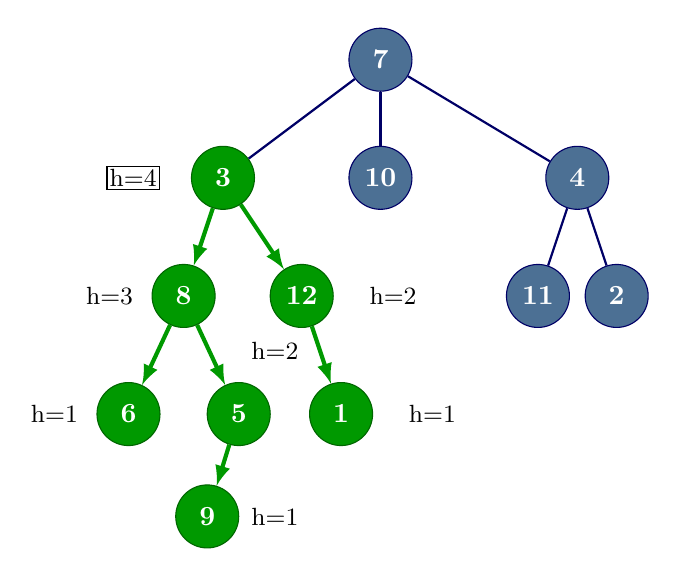
\begin{tikzpicture}[
                % Style giống hệt mẫu bạn cung cấp
                stdnode/.style={circle, draw=blue!40!black, fill=HUSTBlue!70, text=white, font=\bfseries, minimum size=0.8cm, inner sep=0pt},
                highlightnode/.style={circle, draw=green!40!black, fill=green!60!black, text=white, font=\bfseries, minimum size=0.8cm, inner sep=0pt},
                % Style cạnh
                edge/.style={draw=blue!40!black, thick},
                arrowedge/.style={->, >=latex, draw=green!60!black, line width=1.5pt},
                % Style nhãn
                hlabel/.style={draw=white, text=black, fill=white, font=\small, anchor=east, inner sep=1pt}
            ]
                % --- VẼ CÂY ---
                % Root
                \node[stdnode] (n7) at (0, 0) {7};

                % Level 2
                \node[highlightnode] (n3) at (-2, -1.5) {3}; % Đã xong (Xanh)
                \node[stdnode] (n10) at (0, -1.5) {10};
                \node[stdnode] (n4) at (2.5, -1.5) {4};

                % Level 3
                \node[highlightnode] (n8) at (-2.5, -3) {8};   % Đã xong (Xanh)
                \node[highlightnode] (n12) at (-1, -3) {12};  % Đã xong (Xanh)
                \node[stdnode] (n11) at (2, -3) {11};
                \node[stdnode] (n2) at (3, -3) {2};

                % Level 4
                \node[highlightnode] (n6) at (-3.2, -4.5) {6}; % Đã xong (Xanh)
                \node[highlightnode] (n5) at (-1.8, -4.5) {5}; % Đã xong (Xanh)
                \node[highlightnode] (n1) at (-0.5, -4.5) {1}; % Đã xong (Xanh)

                % Level 5 (Node 9)
                \node[highlightnode] (n9) at (-2.2, -5.8) {9}; % Đã xong (Xanh)

                % --- VẼ CẠNH ---
                % Cạnh thường (chưa duyệt)
                \draw[edge] (n7) -- (n3); \draw[edge] (n7) -- (n10); \draw[edge] (n7) -- (n4);
                \draw[edge] (n4) -- (n11); \draw[edge] (n4) -- (n2);

                % Cạnh đệ quy (Mũi tên xanh) - Toàn bộ cây con gốc 3 đã duyệt xong
                \draw[arrowedge] (n3) -- (n8);
                \draw[arrowedge] (n8) -- (n6);
                \draw[arrowedge] (n8) -- (n5);
                \draw[arrowedge] (n5) -- (n9);
                
                \draw[arrowedge] (n3) -- (n12);
                \draw[arrowedge] (n12) -- (n1);

                % --- NHÃN (LABELS) ---
                % Node 3: Kết quả max(3, 2) + 1 = 4
                \node[hlabel, draw=black] at (-2.8, -1.5) {h=4};
                
                % Node 8: h=3
                \node[hlabel] at (-3.1, -3) {h=3};
                
                % Các con của 8
                \node[hlabel, anchor=east] at (-3.8, -4.5) {h=1}; % Node 6
                \node[hlabel, anchor=east] at (-1, -3.7) {h=2}; % Node 5
                \node[hlabel, anchor=east] at (-1, -5.8) {h=1}; % Node 9
                
                % Nhánh 12: Đã có kết quả
                \node[hlabel, anchor=east] at (0.5, -3) {h=2}; % Node 12
                \node[hlabel, anchor=east] at (1, -4.5) {h=1}; % Node 1

            \end{tikzpicture}
            }
        \end{column}
        
        % --- CỘT PHẢI: CODE ---
        \begin{column}{0.5\textwidth}
            \newsavebox{\codeboxHeightFour}
            \begin{lrbox}{\codeboxHeightFour}
                \begin{minipage}{0.95\textwidth}
                    \vspace{0.1cm}
                    \begin{minted}[fontsize=\scriptsize, breaklines]{cpp}
int height(Node* p){
   if(p == NULL) return 0;
   int maxh = 0;
   Node* q = p->leftMostChild;
   while(q != NULL){
      int h = height(q);
      if(h > maxh) maxh = h;
      q = q->rightSibling;
   }
   return maxh + 1;
}
                    \end{minted}
                \end{minipage}
            \end{lrbox}

            \setlength{\fboxrule}{0.8pt}
            \fcolorbox{HUSTBlue}{white}{\usebox{\codeboxHeightFour}}
        \end{column}
    \end{columns}
\end{frame}

\begin{frame}[fragile]{2. THUẬT TOÁN TÌM CHIỀU CAO VÀ ĐỘ SÂU}
    \textbf{2.2. Tìm độ sâu của một nút}
    \begin{itemize}
        \item Độ sâu của một nút
    \end{itemize}

    % Khai báo hộp chứa code
    \newsavebox{\codeboxDepth}
    \begin{lrbox}{\codeboxDepth}
        \begin{minipage}{0.95\textwidth}
            \vspace{0.1cm}
            \begin{minted}[fontsize=\scriptsize, breaklines]{cpp}
int depth(Node* r, int v, int d){
   // d la do sau cua nut r
   if(r == NULL) return -1;
   if(r->id == v) return d;
   Node* p = r->leftMostChild;
   while(p != NULL){
      if(p->id == v) return d+1;
      int dv = depth(p,v,d+1);
      if(dv > 0) return dv;
      p = p->rightSibling;
   }
   return -1;
}
int find_depth(Node* r, int v){
   return depth(r,v,1);
}
            \end{minted}
        \end{minipage}
    \end{lrbox}

    \begin{columns}[T]
        % --- CỘT TRÁI: HÌNH MINH HỌA ---
        \begin{column}{0.5\textwidth}
            \centering
            % Xóa dòng trống trong resizebox để tránh lỗi
            \resizebox{1.0\textwidth}{!}{%
            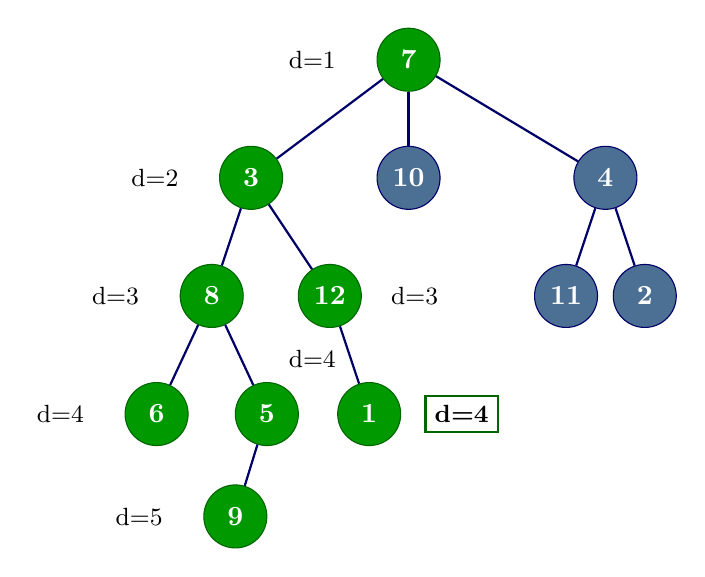
\begin{tikzpicture}[
                % Style nút thường (Xanh dương)
                stdnode/.style={circle, draw=blue!40!black, fill=HUSTBlue!70, text=white, font=\bfseries, minimum size=0.8cm, inner sep=0pt},
                % Style nút được duyệt (Xanh lá)
                highlightnode/.style={circle, draw=green!40!black, fill=green!60!black, text=white, font=\bfseries, minimum size=0.8cm, inner sep=0pt},
                % Style cạnh
                edge/.style={draw=blue!40!black, thick},
                % Style nhãn d=...
                dlabel/.style={font=\small, text=black, anchor=east}
            ]
                % --- VẼ CÂY (Tọa độ thủ công như mẫu) ---
                % Root
                \node[highlightnode] (n7) at (0, 0) {7};

                % Level 2
                \node[highlightnode] (n3) at (-2, -1.5) {3};
                \node[stdnode] (n10) at (0, -1.5) {10};
                \node[stdnode] (n4) at (2.5, -1.5) {4};

                % Level 3
                \node[highlightnode] (n8) at (-2.5, -3) {8};
                \node[highlightnode] (n12) at (-1, -3) {12};
                \node[stdnode] (n11) at (2, -3) {11};
                \node[stdnode] (n2) at (3, -3) {2};

                % Level 4
                \node[highlightnode] (n6) at (-3.2, -4.5) {6};
                \node[highlightnode] (n5) at (-1.8, -4.5) {5};
                \node[highlightnode] (n1) at (-0.5, -4.5) {1}; % Nút cần tìm

                % Level 5
                \node[highlightnode] (n9) at (-2.2, -5.8) {9};

                % --- VẼ CẠNH ---
                \draw[edge] (n7) -- (n3); \draw[edge] (n7) -- (n10); \draw[edge] (n7) -- (n4);
                \draw[edge] (n3) -- (n8); \draw[edge] (n3) -- (n12);
                \draw[edge] (n4) -- (n11); \draw[edge] (n4) -- (n2);
                \draw[edge] (n8) -- (n6); \draw[edge] (n8) -- (n5);
                \draw[edge] (n12) -- (n1);
                \draw[edge] (n5) -- (n9);

                % --- NHÃN (LABELS) ---
                % Các nhãn d=... nằm bên trái
                \node[dlabel] at (-0.8, 0) {d=1};
                \node[dlabel] at (-2.8, -1.5) {d=2};
                \node[dlabel] at (-3.3, -3) {d=3};
                \node[dlabel] at (0.5, -3) {d=3};
                
                \node[dlabel] at (-4.0, -4.5) {d=4};
                \node[dlabel] at (-0.8, -3.8) {d=4};
                
                \node[dlabel] at (-3.0, -5.8) {d=5};

                % Nhãn kết quả d=4 cho nút 1 (trong khung)
                \node[draw=green!40!black, thick, text=black, fill=white, font=\bfseries\small, anchor=west] at (0.2, -4.5) {d=4};

            \end{tikzpicture}%
            }
        \end{column}
        
        % --- CỘT PHẢI: CODE ---
        \begin{column}{0.5\textwidth}
            \setlength{\fboxrule}{0.8pt}
            \fcolorbox{HUSTBlue}{white}{\usebox{\codeboxDepth}}
        \end{column}
    \end{columns}
\end{frame}

	% Slide kết thúc
	{\HUSTUseBackground{theme_hust_oneside.pdf}
		\begin{frame}
			\ifdefstring{\insertaspectratio}{169}{
				\placecontent{0.355\paperwidth}{0.410\paperheight}{0.640\paperwidth}{
					\color{HUSTRed}\bfseries\fontsize{28pt}{36pt}\selectfont\centering
					THANK YOU!
				}
			}{}
		\end{frame}
	}

\end{document}